%
% File: chap04.tex
% Author: Your Name
% Description: Conclusion
%
\let\textcircled=\pgftextcircled
\chapter{Research results}
\label{chap:intro}

\section{Verification of Model Assumptions}

\initial{T}he purpose of this section is to provide a discussion of the potential violation of the underlying assumptions in our research design.

\begin{enumerate}
    \item \textbf{CIA}: This assumption is not statistically verifiable and therefore can only be defended in words. Given the circumstances, we did our best to include the major confounding factors that determine treatment and outcome. However, we must recognize that there may be confounding that we cannot observe. For instance, one could argue that management incentives have a critical impact on treatment and outcome. In particular, incentives that translate into marketing efforts, especially in terms of green washing.

    \item \textbf{Common Support}: This assumption can be statistically tested by calculating the propensity scores for each group and visually checking whether the distribution of propensity scores overlaps in the two groups. In addition, the distributions should also have a similar shape. We show these plots in the analysis, where we also comment on whether the assumption of common support is met.
    
    \item \textbf{SUTVA}: Using reasoning, we can test whether the following two statements are true: (1) the outcome of one observation does not depend on the treatment values of other observations and (2) there are no variations in the treatment of each observation. The first statement could be violated if an issuer has already issued a green bond and concluded that green bond issuance is financially advantageous compared to a conventional bond. If this reasoning leads to more green bonds being issued, it could have an impact on the yield (outcome) of those bonds. However, it is not clear how the overall equilibrium will adjust. We argue that for spillover effects to occur, a significant number of issuers must share the same reasoning at the same time. With respect to the second statement, one could argue that there are different shades of green bonds and, more importantly, that the green bond labelling is not a standardized and unbiased process. However, we argue that we only measure whether a bond is green or not according to Eikon Refinitiv, which in turn relies on the CBI dataset, from which we conclude that we only consider one expert opinion. Thus, we infer that our dataset does not contain variations due to different expert opinions, thereby confirming the validity of the second statement.

    \item \textbf{Exogeneity}: The last assumption of the selection-on-observables study design assumes that the covariates are not affected by the treatment. In this case, one could argue that green bonds tend to finance larger projects and have a longer-term nature than conventional bonds because of their green vision. However, in examining the numbers, we cannot confirm the hypothesis for project size. From a central tendency perspective, conventional bonds finance larger projects. On the other hand, the maturity of green bonds is on average 1.5 years longer compared to their counterparts.
    
    \item \textbf{i.i.d Assumption}: The analysis method used in this paper is only valid under the i.i.d assumption. Due to the fact that our analysis includes the output of different issuers, we cannot assume that the offer yield to maturity follows this assumption. To examine the consequences of violating this assumption on our method, we have provided a small simulation study at the end of this chapter.
\end{enumerate}

\section{Descriptive Statistics}

As an important preliminary note, we will present the descriptive statistics of the universe dataset only. The descriptive statistics of the subsets are presented in the appendix (\ref{desc2},\ref{desc3},\ref{desc4}). Our universe includes a total of 11'179 bonds, of which 9.16\% are green bonds (1'024). These bonds are issued by 2'177 unique issuers. Table \ref{greensum} and Table \ref{brownsum} present the summary statistics for the numerical variables of green and brown bonds, respectively. First, we notice that the maturity of green bonds is on average $533$ days ($\approx 1.5$ years) longer than that of their brown counterpart. Second, the green bond amount issued, on average, is $\approx$ 170\$ million lower than for brown bonds, and green bonds also consist of the zero-coupon type, which is not the case for brown bonds. In addition, the coupon rate for green bonds is $\approx 1\%$ lower than that of brown bonds and the former can even achieve negative values. Finally, the offered yield to maturity for brown bonds is, on average, about 1\% higher than for green bonds. For a more detailed analysis, we have included raincloud plots in the appendix (\ref{rc}).

\begin{table}[!htbp] \centering 
  \caption{Universe Green Bond Numeric Variables Summary Statistics} 
  \label{greensum} 
  \small
\begin{tabular}{@{\extracolsep{5pt}}lccccccc} 
\\[-1.8ex]\hline 
\hline \\[-1.8ex] 
Statistic & \multicolumn{1}{c}{N} & \multicolumn{1}{c}{Mean} & \multicolumn{1}{c}{St. Dev.} & \multicolumn{1}{c}{Min} & \multicolumn{1}{c}{Max} \\ 
\hline \\[-1.8ex] 
Time to Maturity (Days) & 1,024 & 3,214 & 2,418 & 367 & 1,834 & 3,660 & 21,922 \\ 
Issue Amount & 1,024 & 1,290 & 1,960 & 500 & 577 & 1,179 & 33,564 \\ 
Coupon Rate & 1,024 & 1.644 & 1.517 & 0 & 0.5 & 2.4 & 10 \\ 
Offer Yield to Maturity & 1,024 & 1.688 & 1.521 & 0 & 0.5 & 2.5 & 10 \\ 
\hline \\[-1.8ex] 
\end{tabular} 
\end{table}

\begin{table}[!htbp] \centering 
  \caption{Universe Brown Bond Numeric Variables Summary Statistics} 
  \label{brownsum} 
  \small
\begin{tabular}{@{\extracolsep{5pt}}lccccccc} 
\\[-1.8ex]\hline 
\hline \\[-1.8ex] 
Statistic & \multicolumn{1}{c}{N} & \multicolumn{1}{c}{Mean} & \multicolumn{1}{c}{St. Dev.} & \multicolumn{1}{c}{Min} & \multicolumn{1}{c}{Max} \\ 
\hline \\[-1.8ex] 
Time to Maturity (Days) & 11,179 & 2,681 & 2,347.479 & 366 & 1,712 & 3,656 & 36,533 \\ 
Issue Amount & 11,179 & 1,463 & 1,409.418 & 500 & 674 & 1,603 & 30,089 \\ 
Coupon Rate & 11,179 & 2.688 & 1.961 & 0 & 1.1 & 3.9 & 20 \\ 
Offer Yield to Maturity & 11,179 & 2.720 & 1.969 & 0 & 1.1 & 4.0 & 20 \\ 
\hline \\[-1.8ex] 
\end{tabular} 
\end{table} 

Table \ref{propyear} shows the propensities for the year of issuance. For green bonds, the same pattern is observed as in Figure \ref{evo1}: the market grows exponentially every two years until 2021. In contrast, the brown bond market has contracted after 2012 and more than halved by 2021. In addition, our dataset does not include green bonds issued in 2008. Next, in Table \ref{proprating} we show the propensity table for ratings. It can be observed that most green bonds (27\%) are rated triple B, while most brown bonds (36.3\%) are rated triple A. Overall, both green and brown bonds in our dataset are rated at least triple B at 93.5\% and 93.7\%, respectively. For the remaining dummy variables, we will present the propensity tables in the appendix (\ref{PROP}) and only briefly comment on them here. The reason is that their propensities do not show relevant large differences between green and brown bonds, so we can save some space. First, the coupon frequency with the highest frequency is the annual coupon (61\% green, 58\% brown) followed by the semi annual coupon (38.7\% green, 41.6\% brown). The industry for both types of bonds is dominated by financials (48.4\% green, 68.9\% brown) and succeeded by government activity (14.3\% green, 17.1\% brown). One important difference is that the propensity for utilities is higher for green bonds (12.5\%), than for brown bonds (2\%). The Euro market dominates in both bond types (56\% green, 48.2\% brown) followed by the Dollar market (35.9\% green, 39.9\% brown). Regarding seniority, senior unsecured bonds rank prominently for both bond types (72.3\% green, 62.2\% brown). Finally, both types of bonds are balanced in terms of issuer sector and guarantor. In the former, the corporate sector accounts for around $\frac{2}{3}$ of the pie and the public sector for around $\frac{1}{3}$, while in the latter, around 20\% of bonds have a guarantor and around 80\% do not. 

\begin{table}{
    \begin{subtable}{.5\textwidth}
    \centering
        {\begin{tabular}{lll}
        \\[-1.8ex]\hline 
        \hline \\[-1.8ex] 
        \textbf{Issue Year} & \textbf{Green (\%)} & \textbf{Brown (\%)} \\
        \hline \\[-1.8ex]
        {\color[HTML]{333333} 2008} & \cellcolor[HTML]{FFFFFF}{\color[HTML]{333333} 0.0} & \cellcolor[HTML]{9DBC92}{\color[HTML]{333333} 5.9} \\
        {\color[HTML]{333333} 2009} & \cellcolor[HTML]{FCFDFC}{\color[HTML]{333333} 0.3} & \cellcolor[HTML]{1B6C12}{\color[HTML]{FFFFFF} 9.0} \\
        {\color[HTML]{333333} 2010} & \cellcolor[HTML]{FBFCFA}{\color[HTML]{333333} 0.5} & \cellcolor[HTML]{3A7B2D}{\color[HTML]{FFFFFF} 8.4} \\
        {\color[HTML]{333333} 2011} & \cellcolor[HTML]{FFFFFF}{\color[HTML]{333333} 0.0} & \cellcolor[HTML]{4F8841}{\color[HTML]{FFFFFF} 7.9} \\
        {\color[HTML]{333333} 2012} & \cellcolor[HTML]{F9FBF8}{\color[HTML]{333333} 0.7} & \cellcolor[HTML]{006400}{\color[HTML]{FFFFFF} 9.3} \\
        {\color[HTML]{333333} 2013} & \cellcolor[HTML]{F3F7F1}{\color[HTML]{333333} 1.4} & \cellcolor[HTML]{5B8F4D}{\color[HTML]{FFFFFF} 7.6} \\
        {\color[HTML]{333333} 2014} & \cellcolor[HTML]{F6F9F5}{\color[HTML]{333333} 1.0} & \cellcolor[HTML]{5B8F4D}{\color[HTML]{FFFFFF} 7.6} \\
        {\color[HTML]{333333} 2015} & \cellcolor[HTML]{DFE9DB}{\color[HTML]{333333} 3.7} & \cellcolor[HTML]{639555}{\color[HTML]{333333} 7.4} \\
        {\color[HTML]{333333} 2016} & \cellcolor[HTML]{D8E4D3}{\color[HTML]{333333} 4.5} & \cellcolor[HTML]{7AA46D}{\color[HTML]{333333} 6.8} \\
        {\color[HTML]{333333} 2017} & \cellcolor[HTML]{C7D9C0}{\color[HTML]{333333} 6.5} & \cellcolor[HTML]{91B486}{\color[HTML]{333333} 6.2} \\
        {\color[HTML]{333333} 2018} & \cellcolor[HTML]{BDD2B5}{\color[HTML]{333333} 7.7} & \cellcolor[HTML]{A8C49F}{\color[HTML]{333333} 5.6} \\
        {\color[HTML]{333333} 2019} & \cellcolor[HTML]{9BBB90}{\color[HTML]{333333} 11.7} & \cellcolor[HTML]{8DB181}{\color[HTML]{333333} 6.3} \\
        {\color[HTML]{333333} 2020} & \cellcolor[HTML]{729F64}{\color[HTML]{333333} 16.6} & \cellcolor[HTML]{CBDCC5}{\color[HTML]{333333} 4.7} \\
        {\color[HTML]{333333} 2021} & \cellcolor[HTML]{006400}{\color[HTML]{FFFFFF} 27.1} & \cellcolor[HTML]{EBF1E8}{\color[HTML]{333333} 3.9} \\
        {\color[HTML]{333333} 2022} & \cellcolor[HTML]{639556}{\color[HTML]{333333} 18.3} & \cellcolor[HTML]{FFFFFF}{\color[HTML]{333333} 3.4} \\
        \hline \\[-1.8ex]
        \end{tabular}}
    \subcaption{Issue Year}
    \label{propyear}
    \end{subtable}
    \begin{subtable}{0.3\linewidth}
    \centering
        {\begin{tabular}{lll}
        \\[-1.8ex]\hline 
        \hline \\[-1.8ex] 
        \textbf{Rating} & \textbf{Green (\%)} & \textbf{Brown (\%)} \\
        \hline \\[-1.8ex]
        AAA & \cellcolor[HTML]{27711C}{\color[HTML]{FFFFFF} 24.70} & \cellcolor[HTML]{006400}{\color[HTML]{FFFFFF} 36.30} \\
        AA & \cellcolor[HTML]{659658}18.00 & \cellcolor[HTML]{709E63}22.50 \\
        A & \cellcolor[HTML]{317625}{\color[HTML]{FFFFFF} 23.80} & \cellcolor[HTML]{87AD7B}18.90 \\
        BBB & \cellcolor[HTML]{006400}{\color[HTML]{FFFFFF} 27.00} & \cellcolor[HTML]{99B98E}16.00 \\
        BB & \cellcolor[HTML]{D5E3D0}4.80 & \cellcolor[HTML]{E6EEE3}3.90 \\
        \rowcolor[HTML]{F2F6F0} 
        B & 1.50 & 2.10 \\
        CCC & \cellcolor[HTML]{FFFFFF}0.02 & \cellcolor[HTML]{FFFFFF}0.03 \\
        \hline \\[-1.8ex]
        \end{tabular}}
    \subcaption{Rating}
    \label{proprating}
    \end{subtable}
\caption{Propensity Tables}}
\end{table}

Another important preliminary analysis should be performed with respect to correlations. Since our dataset contains too many variables to display a correlation heatmap, in Figure \ref{corr} we show the 10 most relevant pairs according to the highest correlation at a statistical p-value below 5\%. Strikingly, we have a highly correlated pair, namely the coupon rate with our outcome variable, which is 99\% correlated. Because of the high correlation, we run the risk that the Random Forest method often uses this variable as a split variable, making the Leafs no longer heterogeneous and driving the effect to zero. Indeed, the analysis showed that the majority of splits are caused by the coupon rate, and adjusting the hyperparameters did not solve the problem.\footnote{We do not report this result in this paper. However, one can increase the number of \textit{mtry}. This hyperparameter determines the number of variables that are considered as split candidates within a tree. Thus, with a higher number, the probability of selecting our highly correlated variable decreases. Similarly, one can enable the algorithm to tune a set of hyperparameters by cross-validation.} Due to the fact that the coupon rate is very closely related to the offer yield to maturity but theoretically does not influence the choice of treatment and therefore cannot be interpreted as a confounder, we exclude this variable in our specifications.\footnote{For example, if a 1-year bond with a 4\% coupon rate and a face value of 100 is sold for 100 (at par) in the market, the issue yield is also 4\%. In case the issuer decides to grant a discount, the issue yield must be greater than the coupon rate. Vice versa, if the bond sells at a premium, issue yield < coupon rate.} The remaining pairs are correlations between covariates. In this case, each of these correlated features can be used as a predictor without favoring one over the others. To verify this, take for example the fourth pair, which displays a correlation of about 75\% between euro- and U.S. dollar-denominated bonds. When splitting a tree, sometimes the Euro is used and sometimes the U.S. dollar, which leads to a distortion of their importance. Therefore, caution should be exercised when interpreting the results.

\begin{figure}[ht!]
    \centering
    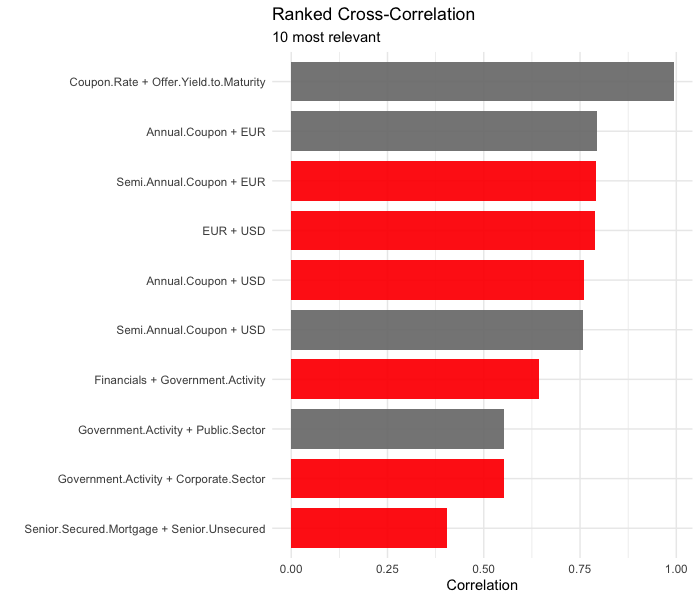
\includegraphics[scale=0.5]{chinchilab-template/chapters/chapter04/correlation1.png}
    \caption{Ranked Cross-Correlation of 10 Most Relevant Pairs.}
    \caption*{Note: Grey = Positive Correlation, Red = Negative Correlation.}
    \label{corr}
\end{figure}

\newpage

\section{Causal Forest Analysis}

Our analysis consists of four data sets and three different methodological specifications. Based on these, we analyzed a total of 11 different models. To present them all in this paper is beyond the scope of readability and comprehensibility. Therefore, we select the two most relevant models to present in this chapter and report the results of the remaining models in the appendix. When deemed adequate, we refer the reader to the appendix. 

Table \ref{tabate} provides an overview of the ATE estimates for the 11 models. The first distinct observation we draw is that all of our models show a negative average treatment effect, supporting the greenium hypothesis. These estimates range from -0.186\% to -1.032\%, or, in financial jargon, from 18.6 to 103.2 basis points. The central tendency of this sample of ATEs is -0.43\%. These results are of great significance not only in statistical terms, but also in economic terms. An important note is that the estimates of the models without issuer controls should only be interpreted for the sake of comparison with the methods which include issuer controls. Interestingly, we find that in all of our four data sets, the ATE estimate increases in magnitude when issuer controls are included. Furthermore, PSM Zerbib stands for Propensity Score Matching, which includes the variables proposed by \citet{zerbib2017green}. The matching is performed for each issuer cluster before the causal forest analysis. Therefore, we suggest that this method provides the best performance in terms of robustness.

\begin{table}[h!] \centering
\footnotesize
\caption{ATE across Models}
\label{tabate}
\begin{tabular}{
>{\columncolor[HTML]{FFFFFF}}r 
>{\columncolor[HTML]{FFFFFF}}r rr}
\\[-1.8ex]\hline 
\hline \\[-1.8ex] 
\cellcolor[HTML]{FFFFFF}{\color[HTML]{333333} Dataset} & \cellcolor[HTML]{FFFFFF}{\color[HTML]{333333} Method} & \cellcolor[HTML]{FFFFFF}{\color[HTML]{333333} ATE Estimate} & \cellcolor[HTML]{FFFFFF}{\color[HTML]{333333} ATE Std. Err.} \\ \hline
{\color[HTML]{333333} Data Universe} & {\color[HTML]{333333} Without Issuer Controls} & \cellcolor[HTML]{DBF1D5}{\color[HTML]{333333} -0.3175919} & {\color[HTML]{333333} 0.02069961} \\ \cline{2-4} 
{\color[HTML]{333333} Data Universe} & {\color[HTML]{333333} With Issuer Controls} & \cellcolor[HTML]{00441B}{\color[HTML]{FFFFFF} -1.0322041} & {\color[HTML]{333333} 0.04456669} \\ \hline
{\color[HTML]{333333} Data Matched} & {\color[HTML]{333333} Without Issuer Controls} & \cellcolor[HTML]{F5FBF3}{\color[HTML]{333333} -0.1857373} & {\color[HTML]{333333} 0.02581946} \\ \cline{2-4} 
{\color[HTML]{333333} Data Matched} & {\color[HTML]{333333} With Issuer Controls} & \cellcolor[HTML]{7CC77C}{\color[HTML]{333333} -0.5854021} & {\color[HTML]{333333} 0.02749895} \\ \cline{2-4} 
\cellcolor[HTML]{FFFFFF}{\color[HTML]{333333} Data Matched} & \cellcolor[HTML]{FFFFFF}{\color[HTML]{333333} PSM Zerbib} & \cellcolor[HTML]{D4EECD}{\color[HTML]{333333} -0.3431900} & {\color[HTML]{333333} 0.05963097} \\ \hline
{\color[HTML]{333333} USDEUR Matched} & {\color[HTML]{333333} Without Issuer Controls} & \cellcolor[HTML]{F7FCF5}{\color[HTML]{333333} -0.1740170} & {\color[HTML]{333333} 0.02782810} \\ \cline{2-4} 
{\color[HTML]{333333} USDEUR Matched} & {\color[HTML]{333333} With Issuer Controls} & \cellcolor[HTML]{8DCF8A}{\color[HTML]{333333} -0.5445872} & {\color[HTML]{333333} 0.02776807} \\ \cline{2-4} 
\cellcolor[HTML]{FFFFFF}{\color[HTML]{333333} USDEUR Matched} & \cellcolor[HTML]{FFFFFF}{\color[HTML]{333333} PSM Zerbib} & \cellcolor[HTML]{E0F3DB}{\color[HTML]{333333} -0.2975631} & {\color[HTML]{333333} 0.05195736} \\ \hline
{\color[HTML]{333333} CBI Matched} & {\color[HTML]{333333} Without Issuer Controls} & \cellcolor[HTML]{E9F7E5}{\color[HTML]{333333} -0.2558610} & {\color[HTML]{333333} 0.03095115} \\ \cline{2-4} 
{\color[HTML]{333333} CBI Matched} & {\color[HTML]{333333} With Issuer Controls} & \cellcolor[HTML]{A2D99C}{\color[HTML]{333333} -0.4943476} & {\color[HTML]{333333} 0.03200607} \\ \cline{2-4} 
\cellcolor[HTML]{FFFFFF}{\color[HTML]{333333} CBI Matched} & \cellcolor[HTML]{FFFFFF}{\color[HTML]{333333} PSM Zerbib} & \cellcolor[HTML]{9FD89A}{\color[HTML]{333333} -0.4999409} & {\color[HTML]{333333} 0.06891475} \\ \hline
\end{tabular}
\end{table}

Figure \ref{figate} illustrates the ATE estimates and shows in dark green the two models we present in the following analysis. The reason we select them over the others is that the specifications of models (1) through (3) as well as (6) and (9) are less robust. Moreover, we can easily compare these two models with the models of the other two subsets.


\begin{figure}[h!]
    \centering
    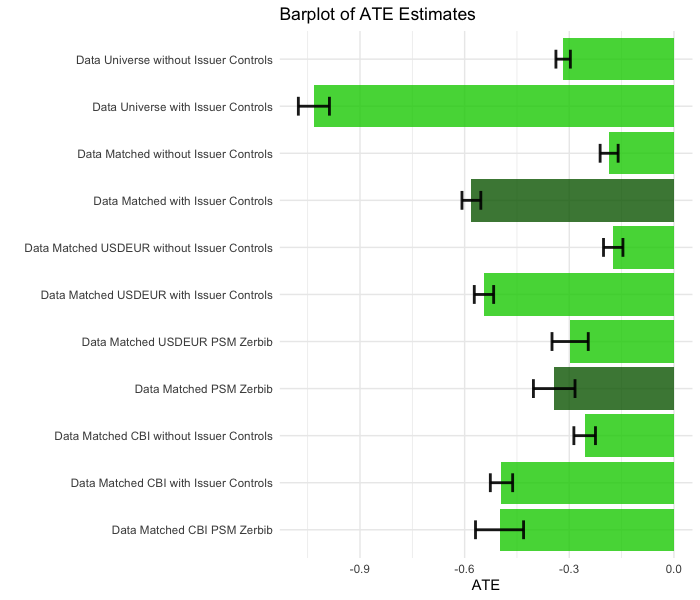
\includegraphics[scale=0.45]{chinchilab-template/chapters/chapter04/ate_barplot.png}
    \caption{Barplot of ATE Estimates}
    \label{figate}
\end{figure}


%%%%%%%%%%%%%%%%%%%%%%%%%%%%%%%%%%%%%%%%%%%%%%%%%%%%%%%%%%%%
\subsection{Data Matched with Issuer Controls}
%%%%%%%%%%%%%%%%%%%%%%%%%%%%%%%%%%%%%%%%%%%%%%%%%%%%%%%%%%%%


%%%%%%%%%%%%%%%%%%%%%%%%%%%%%%%%%%%%%%%%%%%%%%%%%%%%%%%%%%%%
\subsubsection*{Nuisance Parameter Check}
%%%%%%%%%%%%%%%%%%%%%%%%%%%%%%%%%%%%%%%%%%%%%%%%%%%%%%%%%%%%

First, we perform calibration checks to ensure that the nuisance parameters are well calibrated and that the propensity scores are sufficiently bounded from 0 and 1 and have adequate overlap. The latter checks the assumption of common support. The following calibration regressions are deployed to evaluate the performance of the propensity and outcome models:

\begin{equation}
W_{i}=\alpha \bar{e}+\beta\left(\hat{e}^{-i}\left(X_{i}\right)-\bar{e}\right)+\epsilon \quad \bar{e}:=\frac{1}{n} \sum_{i=1}^{n} \hat{e}^{-i}\left(X_{i}\right) \quad \text{(Propensity Model)}
\end{equation}

\begin{equation}
W_{i}=\alpha \bar{m}+\beta\left(\hat{m}^{-i}\left(X_{i}\right)-\bar{m}\right)+\epsilon \quad \bar{m}:=\frac{1}{n} \sum_{i=1}^{n} \hat{m}^{-i}\left(X_{i}\right) \quad \text{(Outcome Model)}
\end{equation}

The coefficients $\alpha$ and $\beta$ allow us to evaluate the performance of our estimates. If $\alpha=1$, then the average prediction is correct. If $\beta=1$, then the nuisance parameters adequately capture the underlying heterogeneity \cite{athey}. First, the propensity score distribution is shown in Figure \ref{prop4}. The distributions do not overlap sufficiently, and the shape of the distributions also differs. Thus, we conclude that the assumption of common support is violated to some extent.

Second, the output of the calibration regressions is shown in Table \ref{calibration1}. We conclude that both nuisance parameter estimations are correct in terms of average prediction and also seem to sufficiently capture the underlying heterogeneity.

\begin{figure}[H]
    \centering
    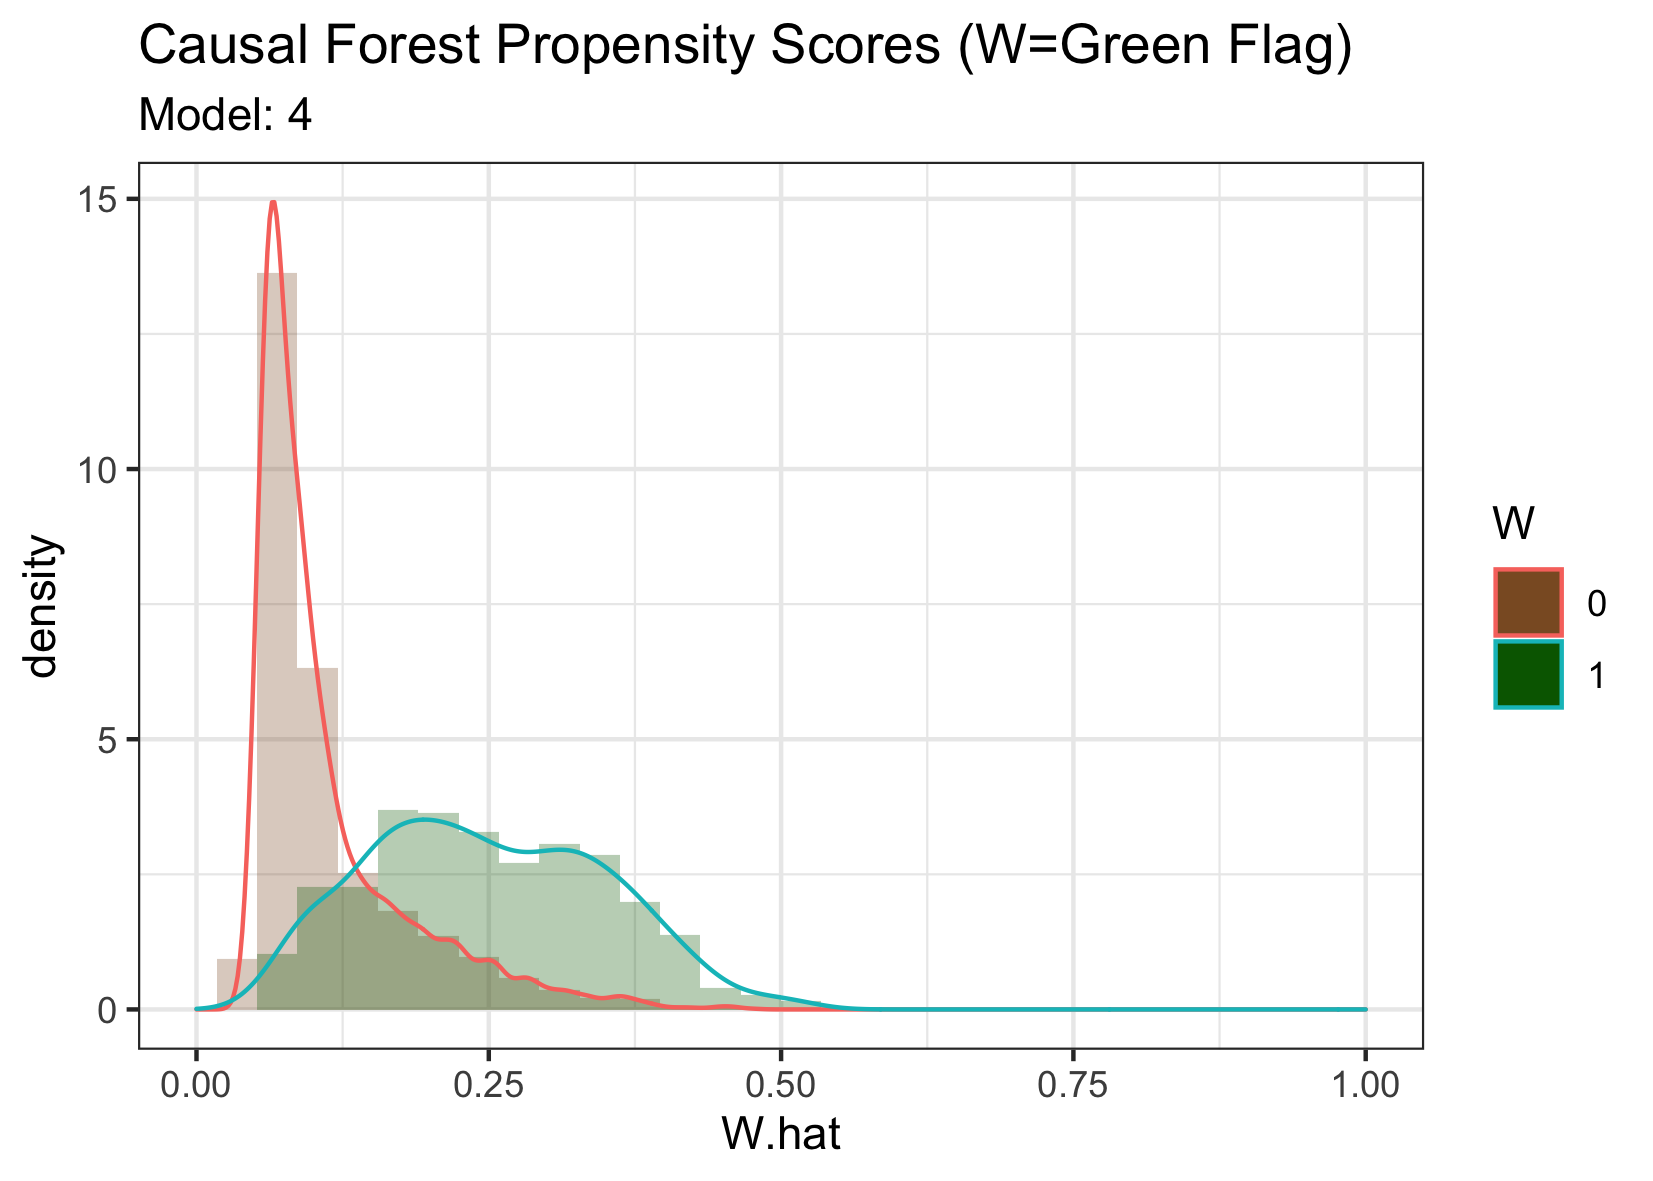
\includegraphics[scale=0.2]{chinchilab-template/chapters/appendices/ANALYSIS/prop_4.png}
    \caption{Propensity Score Distribution (Model 4)}
    \label{prop4}
\end{figure}


\begin{table}[H]{
    \begin{subtable}{.5\textwidth}
    \centering
    \footnotesize
        {\begin{tabular}{@{\extracolsep{5pt}}lc} 
        \\[-1.8ex]\hline 
        \hline \\[-1.8ex] 
         & \multicolumn{1}{c}{\textit{Dependent variable: Green Flag}} \\ 
        \cline{2-2} 
        \\[-1.8ex] &   \\ 
        \hline \\[-1.8ex] 
         e.bar & 0.999$^{***}$ \\ 
          & (0.029) \\ 
          & \\ 
         e.residual & 2.076$^{***}$ \\ 
          & (0.062) \\ 
          & \\ 
        \hline \\[-1.8ex] 
        \hline 
        \hline \\[-1.8ex] 
        \textit{Note:}  & \multicolumn{1}{r}{$^{*}$p$<$0.1; $^{**}$p$<$0.05; $^{***}$p$<$0.01} \\ 
        \end{tabular}}
    \subcaption{Outcome Model}
    \end{subtable}
    \begin{subtable}{0.3\linewidth}
    \centering
    \footnotesize
        {\begin{tabular}{@{\extracolsep{5pt}}lc} 
        \\[-1.8ex]\hline 
        \hline \\[-1.8ex] 
         & \multicolumn{1}{c}{\textit{Dependent variable: Green Flag}} \\ 
        \cline{2-2} 
        \\[-1.8ex] &   \\ 
        \hline \\[-1.8ex] 
         m.bar & 1.000$^{***}$ \\ 
          & (0.011) \\ 
          & \\ 
         m.residual & 2.260$^{***}$ \\ 
          & (0.031) \\ 
          & \\ 
        \hline \\[-1.8ex] 
        \hline 
        \hline \\[-1.8ex] 
        \textit{Note:}  & \multicolumn{1}{r}{$^{*}$p$<$0.1; $^{**}$p$<$0.05; $^{***}$p$<$0.01} \\ 
        \end{tabular}}
    \subcaption{Propensity Model}
    \end{subtable}
\caption{Calibration Regressions (Model 4)}
\label{calibration1}}
\end{table}

%%%%%%%%%%%%%%%%%%%%%%%%%%%%%%%%%%%%%%%%%%%%%%%%%%%%%%%%%%%%
\subsubsection*{Heterogeneity Assessment}
%%%%%%%%%%%%%%%%%%%%%%%%%%%%%%%%%%%%%%%%%%%%%%%%%%%%%%%%%%%%
Another option to examine whether the trained causal forests have detected treatment heterogeneity is to "naively" examine the distribution of the individual CATE predictions. As can be seen in Figure \ref{cate4}, there is a clear trend, indicating that we do have heterogeneity indeed. Moreover, most of the observations lie between -0.75\% and -0.25\%.

\begin{figure}[H]
    \centering
    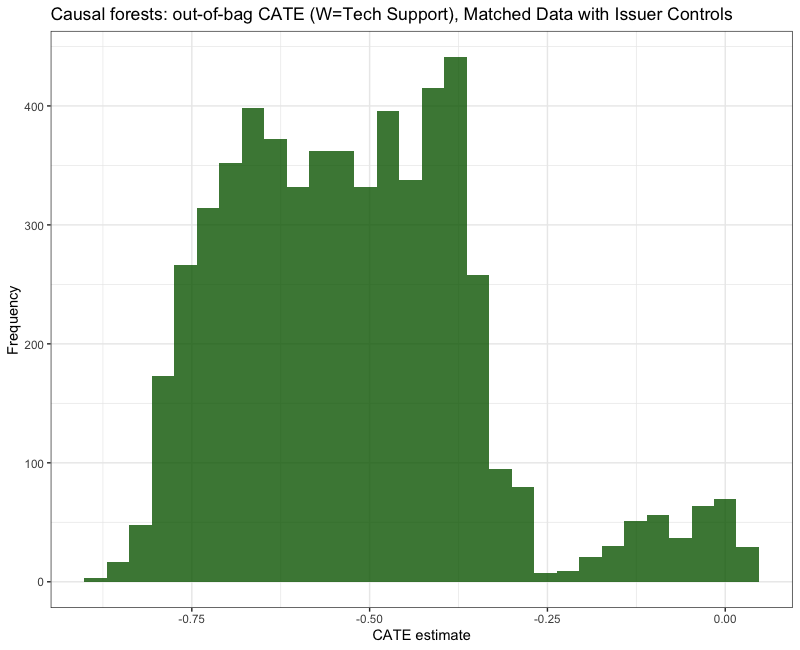
\includegraphics[scale=0.3]{chinchilab-template/chapters/appendices/ANALYSIS/CATE_cf1.1.png}
    \caption{Distribution of CATE (Model 4)}
    \label{cate4}
\end{figure}



The Generalized Random Forest (\textit{grf}) package provides a measure of variable importance, indicating how frequently a variable appeared in a tree split. However, when estimating the importance of variables, a distortion occurs when both continuous and discrete variables are used. This is due to the fact that continuous variables contain a different amount of information than discrete variables. In particular, tree-based methods may be biased in favor of continuous variables due to the larger number of potential split points. This is especially a concern when the discrete variables are of the dummy type \citep[p. 3]{o2018causal}. Besides, the issue of correlation applies here as well. Table \ref{varimp4} should therefore be considered only as a rough indication of the source of heterogeneity.

\begin{table}[h!]
\centering
\caption{Variable Importance (Model 4)}
\label{varimp4}
\begin{tabular}{lr}
\\[-1.8ex]\hline 
\hline \\[-1.8ex]
\rowcolor[HTML]{FFFFFF} 
{\color[HTML]{333333} \textbf{Covariate}} & {\color[HTML]{333333} \textbf{Value} } \\ \hline
\rowcolor[HTML]{FFFFFF} 
{\color[HTML]{333333} 2022} & \cellcolor[HTML]{00441B}{\color[HTML]{FFFFFF} 0.1067} \\
\rowcolor[HTML]{FFFFFF} 
{\color[HTML]{333333} Issue Amount} & \cellcolor[HTML]{006C2C}{\color[HTML]{FFFFFF} 0.0995} \\
\rowcolor[HTML]{FFFFFF} 
{\color[HTML]{333333} Time to Maturity (Days)} & \cellcolor[HTML]{359E53}{\color[HTML]{FFFFFF} 0.0876} \\
\rowcolor[HTML]{FFFFFF} 
{\color[HTML]{333333} Annual Coupon} & \cellcolor[HTML]{DAF1D4}{\color[HTML]{333333} 0.0576} \\
\rowcolor[HTML]{FFFFFF} 
{\color[HTML]{333333} Semi Annual Coupon} & \cellcolor[HTML]{E1F3DB}{\color[HTML]{333333} 0.056} \\
\rowcolor[HTML]{FFFFFF} 
{\color[HTML]{333333} EUR} & \cellcolor[HTML]{F7FCF5}{\color[HTML]{333333} 0.0475} \\ \hline
\end{tabular}
\end{table}

Another approach to synthesize the results of a complex algorithm, such as causal forests, is to form subgroups based on the magnitude of the predicted treatment effect. Compared to variable importance, this method is more descriptive and does not depend on whether a tree splits on a covariate or not. Therefore, it can provide us with valuable insight. With this approach, we divide the data into clusters, based on the n-tiles of the predicted treatment effect. In our case, we chose $n=4$, which means that we look at the quartiles. Then we calculate the average treatment effect within each quartile by using two methods: Sample Average Treatment Effect and Augmented Inverse-Propensity Weighted (AIPW). The latter method is recommended for calculating the average treatment effect for observational data - as is the case in the present study \citep{athey}. Figure \ref{quart4} shows the ATE point estimate with error bounds across four quartiles.

\begin{figure}[h!]
    \centering
    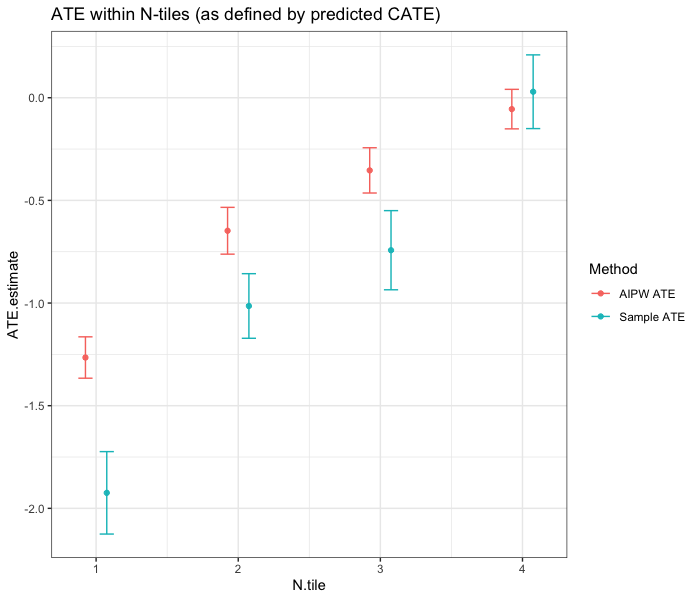
\includegraphics[scale=0.4]{chinchilab-template/chapters/appendices/ANALYSIS/ntiles_cf1.1.png}
    \caption{Graph of ATE within Subgroups (Model 4)}
    \label{quart4}
\end{figure}

To confirm the hypothesis derived from the variable importance table and to assess which covariates influence these varying treatment effects across quantiles and to what extent, Table \ref{Het4} presents the average level of each covariate across all quartiles. First, we observe that green bonds with a longer time to maturity fetch a lower average treatment effect (higher greenium) than shorter ones. Second, green bonds with an annual coupon have higher greenium, while green bonds with a semi-annual coupon have the lowest greenium. Third, green bond issuers from the financial sector tend to achieve lower greenium, while issuers from the technology and utilities sectors achieve the highest greenium. Fourth, euro-denominated green bonds have higher greenium, while U.S. dollar-denominated green bonds have the lowest greenium. And last but not least, green bonds issued from 2013 to 2016 experienced larger greeniums compared to green bonds issued between 2017 and 2022.

Another method to understand the rationale behind our causal forest black box predictions is to analyse partial dependency plots. Thereby we perform a ceteris paribus analysis on the three most important variables according to Table \ref{varimp4} by examining how the CATE estimates behave when we vary our variable of interest while keeping all other covariates fixed at their median. First, Figure \ref{pdp2022} also shows that green bonds issued in 2022 have lower negative treatment effects compared to 2012. Second, the effect of issue amount remains stable. Thus, the isolated effect of issue amount on the treatment effect is approx. zero. However, the isolated effect of time of maturity in Figure \ref{pdpttm} shows a slightly positive effect as already described above.

\begin{figure}[H]
\centering
   \begin{subfigure}[b]{0.45\textwidth} \centering
    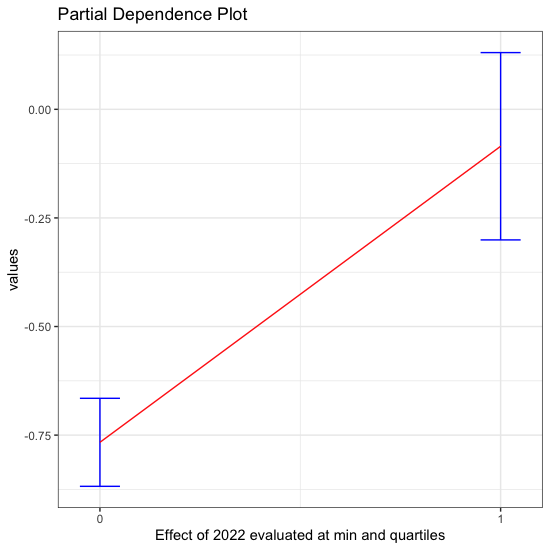
\includegraphics[width=0.65\textwidth]{chinchilab-template/chapters/appendices/ANALYSIS/PDP_cf1.1.png}   
    \caption{Effect of 2022}
    \label{pdp2022} 
\end{subfigure}
\begin{subfigure}[b]{0.5\textwidth} \centering
    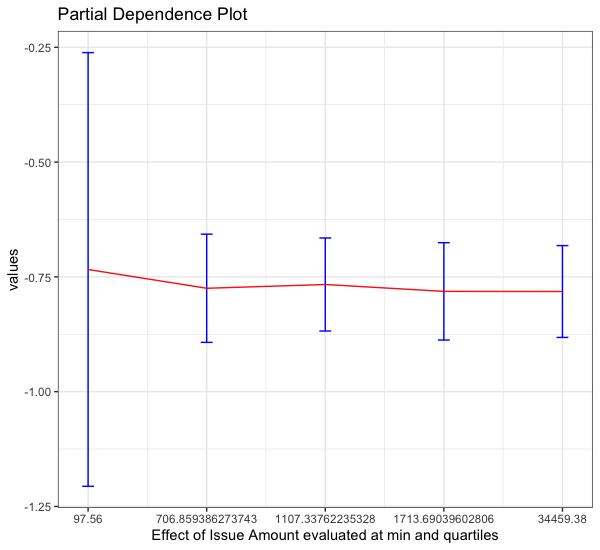
\includegraphics[width=0.65\textwidth]{chinchilab-template/chapters/appendices/ANALYSIS/PDP2_cf1.1.png}
   \caption{Effect of Issue Amount}
   \label{pdpia}
\end{subfigure}
\\
\begin{subfigure}[b]{0.5\textwidth} \centering
    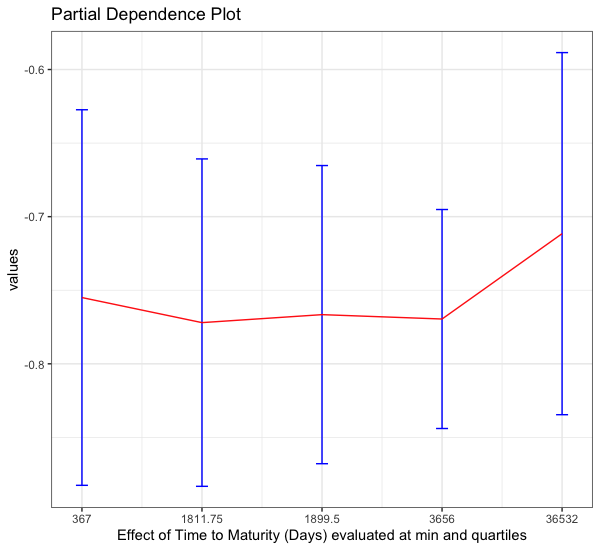
\includegraphics[width=0.65\textwidth]{chinchilab-template/chapters/appendices/ANALYSIS/PDP3_cf1.1.png}
   \caption{Effect of Time to Maturity (Days)}
   \label{pdpttm}
\end{subfigure}
\caption{Partial Dependency Plots (Model 4)}
\end{figure}

\begin{table}[H]
\centering
\caption{Heterogeneity across Covariates (Model 4)}
\label{Het4}
\scriptsize
\begin{tabular}{lllll}
\\[-1.8ex]\hline 
\hline \\[-1.8ex] 
{\color[HTML]{333333} \textbf{Variable}} & {\color[HTML]{333333} \textbf{Mean ntile1}} & {\color[HTML]{333333} \textbf{Mean ntile2}} & {\color[HTML]{333333} \textbf{Mean ntile3}} & {\color[HTML]{333333} \textbf{Mean ntile4}} \\
\hline \\[-1.8ex] 
{\color[HTML]{333333} Time to Maturity (Days)} & \cellcolor[HTML]{A0D7AF}{\color[HTML]{333333} 2857.9} & \cellcolor[HTML]{63BE7B}{\color[HTML]{333333} 3539.32} & \cellcolor[HTML]{9FD7AF}{\color[HTML]{333333} 2865.62} & \cellcolor[HTML]{FCFCFF}{\color[HTML]{333333} 1801.99} \\
{\color[HTML]{333333} Issue Amount} & \cellcolor[HTML]{63BE7B}{\color[HTML]{333333} 1704.89} & \cellcolor[HTML]{B5DFC2}{\color[HTML]{333333} 1543.02} & \cellcolor[HTML]{FCFCFF}{\color[HTML]{333333} 1400.54} & \cellcolor[HTML]{78C78D}{\color[HTML]{333333} 1663.67} \\
{\color[HTML]{333333} Guarantor} & \cellcolor[HTML]{E1F1E8}{\color[HTML]{333333} 0.18} & \cellcolor[HTML]{E1F1E8}{\color[HTML]{333333} 0.18} & \cellcolor[HTML]{E9F4EE}{\color[HTML]{333333} 0.13} & \cellcolor[HTML]{D9EEE1}{\color[HTML]{333333} 0.23} \\
{\color[HTML]{333333} 2013} & \cellcolor[HTML]{ECF6F1}{\color[HTML]{333333} 0.11} & \cellcolor[HTML]{F5F9F9}{\color[HTML]{333333} 0.05} & \cellcolor[HTML]{F3F9F8}{\color[HTML]{333333} 0.06} & \cellcolor[HTML]{F5F9F9}{\color[HTML]{333333} 0.05} \\
{\color[HTML]{333333} 2014} & \cellcolor[HTML]{ECF6F1}{\color[HTML]{333333} 0.11} & \cellcolor[HTML]{F3F9F8}{\color[HTML]{333333} 0.06} & \cellcolor[HTML]{F3F9F8}{\color[HTML]{333333} 0.06} & \cellcolor[HTML]{F6FAFA}{\color[HTML]{333333} 0.04} \\
{\color[HTML]{333333} 2015} & \cellcolor[HTML]{F5F9F9}{\color[HTML]{333333} 0.05} & \cellcolor[HTML]{EFF7F4}{\color[HTML]{333333} 0.09} & \cellcolor[HTML]{EFF7F4}{\color[HTML]{333333} 0.09} & \cellcolor[HTML]{F2F8F6}{\color[HTML]{333333} 0.07} \\
{\color[HTML]{333333} 2016} & \cellcolor[HTML]{F2F8F6}{\color[HTML]{333333} 0.07} & \cellcolor[HTML]{EFF7F4}{\color[HTML]{333333} 0.09} & \cellcolor[HTML]{F2F8F6}{\color[HTML]{333333} 0.07} & \cellcolor[HTML]{F0F8F5}{\color[HTML]{333333} 0.08} \\
{\color[HTML]{333333} 2017} & \cellcolor[HTML]{F9FBFD}{\color[HTML]{333333} 0.02} & \cellcolor[HTML]{EDF6F2}{\color[HTML]{333333} 0.1} & \cellcolor[HTML]{EDF6F2}{\color[HTML]{333333} 0.1} & \cellcolor[HTML]{F2F8F6}{\color[HTML]{333333} 0.07} \\
{\color[HTML]{333333} 2018} & \cellcolor[HTML]{FCFCFF}{\color[HTML]{333333} 0} & \cellcolor[HTML]{F2F8F6}{\color[HTML]{333333} 0.07} & \cellcolor[HTML]{EAF5F0}{\color[HTML]{333333} 0.12} & \cellcolor[HTML]{F0F8F5}{\color[HTML]{333333} 0.08} \\
{\color[HTML]{333333} 2019} & \cellcolor[HTML]{F6FAFA}{\color[HTML]{333333} 0.04} & \cellcolor[HTML]{E9F4EE}{\color[HTML]{333333} 0.13} & \cellcolor[HTML]{EAF5F0}{\color[HTML]{333333} 0.12} & \cellcolor[HTML]{F8FBFC}{\color[HTML]{333333} 0.03} \\
{\color[HTML]{333333} 2020} & \cellcolor[HTML]{FBFCFE}{\color[HTML]{333333} 0.01} & \cellcolor[HTML]{EFF7F4}{\color[HTML]{333333} 0.09} & \cellcolor[HTML]{F0F8F5}{\color[HTML]{333333} 0.08} & \cellcolor[HTML]{F0F8F5}{\color[HTML]{333333} 0.08} \\
{\color[HTML]{333333} 2021} & \cellcolor[HTML]{F6FAFA}{\color[HTML]{333333} 0.04} & \cellcolor[HTML]{EFF7F4}{\color[HTML]{333333} 0.09} & \cellcolor[HTML]{EFF7F4}{\color[HTML]{333333} 0.09} & \cellcolor[HTML]{F3F9F8}{\color[HTML]{333333} 0.06} \\
{\color[HTML]{333333} 2022} & \cellcolor[HTML]{FCFCFF}{\color[HTML]{333333} 0} & \cellcolor[HTML]{FCFCFF}{\color[HTML]{333333} 0} & \cellcolor[HTML]{FCFCFF}{\color[HTML]{333333} 0} & \cellcolor[HTML]{D5ECDD}{\color[HTML]{333333} 0.26} \\
{\color[HTML]{333333} Annual Coupon} & \cellcolor[HTML]{63BE7B}{\color[HTML]{333333} 1} & \cellcolor[HTML]{71C487}{\color[HTML]{333333} 0.91} & \cellcolor[HTML]{B8E1C4}{\color[HTML]{333333} 0.45} & \cellcolor[HTML]{DFF1E6}{\color[HTML]{333333} 0.19} \\
{\color[HTML]{333333} Semi Annual Coupon} & \cellcolor[HTML]{FCFCFF}{\color[HTML]{333333} 0} & \cellcolor[HTML]{EFF7F4}{\color[HTML]{333333} 0.09} & \cellcolor[HTML]{AADBB8}{\color[HTML]{333333} 0.54} & \cellcolor[HTML]{82CB96}{\color[HTML]{333333} 0.8} \\
{\color[HTML]{333333} Quarterly} & \cellcolor[HTML]{FCFCFF}{\color[HTML]{333333} 0} & \cellcolor[HTML]{FCFCFF}{\color[HTML]{333333} 0} & \cellcolor[HTML]{FCFCFF}{\color[HTML]{333333} 0} & \cellcolor[HTML]{FCFCFF}{\color[HTML]{333333} 0} \\
{\color[HTML]{333333} Senior Secured Mortgage} & \cellcolor[HTML]{FCFCFF}{\color[HTML]{333333} 0} & \cellcolor[HTML]{E6F3EC}{\color[HTML]{333333} 0.15} & \cellcolor[HTML]{E9F4EE}{\color[HTML]{333333} 0.13} & \cellcolor[HTML]{F5F9F9}{\color[HTML]{333333} 0.05} \\
{\color[HTML]{333333} Senior Secured} & \cellcolor[HTML]{F8FBFC}{\color[HTML]{333333} 0.03} & \cellcolor[HTML]{F2F8F6}{\color[HTML]{333333} 0.07} & \cellcolor[HTML]{F3F9F8}{\color[HTML]{333333} 0.06} & \cellcolor[HTML]{F3F9F8}{\color[HTML]{333333} 0.06} \\
{\color[HTML]{333333} Senior Unsecured} & \cellcolor[HTML]{7FCA93}{\color[HTML]{333333} 0.82} & \cellcolor[HTML]{9ED6AE}{\color[HTML]{333333} 0.62} & \cellcolor[HTML]{B6E0C3}{\color[HTML]{333333} 0.46} & \cellcolor[HTML]{8DCF9F}{\color[HTML]{333333} 0.73} \\
{\color[HTML]{333333} Senior Non Preferred} & \cellcolor[HTML]{FCFCFF}{\color[HTML]{333333} 0} & \cellcolor[HTML]{FBFCFE}{\color[HTML]{333333} 0.01} & \cellcolor[HTML]{EFF7F4}{\color[HTML]{333333} 0.09} & \cellcolor[HTML]{F9FBFD}{\color[HTML]{333333} 0.02} \\
{\color[HTML]{333333} Senior Preferred} & \cellcolor[HTML]{FCFCFF}{\color[HTML]{333333} 0} & \cellcolor[HTML]{F8FBFC}{\color[HTML]{333333} 0.03} & \cellcolor[HTML]{EAF5F0}{\color[HTML]{333333} 0.12} & \cellcolor[HTML]{F5F9F9}{\color[HTML]{333333} 0.05} \\
{\color[HTML]{333333} Senior Subordinated Unsecured} & \cellcolor[HTML]{FBFCFE}{\color[HTML]{333333} 0.01} & \cellcolor[HTML]{FCFCFF}{\color[HTML]{333333} 0} & \cellcolor[HTML]{FCFCFF}{\color[HTML]{333333} 0} & \cellcolor[HTML]{FCFCFF}{\color[HTML]{333333} 0} \\
{\color[HTML]{333333} Subordinated Unsecured} & \cellcolor[HTML]{FBFCFE}{\color[HTML]{333333} 0.01} & \cellcolor[HTML]{F8FBFC}{\color[HTML]{333333} 0.03} & \cellcolor[HTML]{F6FAFA}{\color[HTML]{333333} 0.04} & \cellcolor[HTML]{FCFCFF}{\color[HTML]{333333} 0} \\
{\color[HTML]{333333} Basic Materials} & \cellcolor[HTML]{FBFCFE}{\color[HTML]{333333} 0.01} & \cellcolor[HTML]{FBFCFE}{\color[HTML]{333333} 0.01} & \cellcolor[HTML]{FCFCFF}{\color[HTML]{333333} 0} & \cellcolor[HTML]{FCFCFF}{\color[HTML]{333333} 0} \\
{\color[HTML]{333333} Consumer Cyclicals} & \cellcolor[HTML]{F9FBFD}{\color[HTML]{333333} 0.02} & \cellcolor[HTML]{FCFCFF}{\color[HTML]{333333} 0} & \cellcolor[HTML]{FCFCFF}{\color[HTML]{333333} 0} & \cellcolor[HTML]{FCFCFF}{\color[HTML]{333333} 0} \\
{\color[HTML]{333333} Consumer Non Cyclicals} & \cellcolor[HTML]{FCFCFF}{\color[HTML]{333333} 0} & \cellcolor[HTML]{FCFCFF}{\color[HTML]{333333} 0} & \cellcolor[HTML]{FCFCFF}{\color[HTML]{333333} 0} & \cellcolor[HTML]{FCFCFF}{\color[HTML]{333333} 0} \\
{\color[HTML]{333333} Energy} & \cellcolor[HTML]{F9FBFD}{\color[HTML]{333333} 0.02} & \cellcolor[HTML]{FCFCFF}{\color[HTML]{333333} 0} & \cellcolor[HTML]{FCFCFF}{\color[HTML]{333333} 0} & \cellcolor[HTML]{FCFCFF}{\color[HTML]{333333} 0} \\
{\color[HTML]{333333} Financials} & \cellcolor[HTML]{AADBB8}{\color[HTML]{333333} 0.54} & \cellcolor[HTML]{9FD7AF}{\color[HTML]{333333} 0.61} & \cellcolor[HTML]{91D1A3}{\color[HTML]{333333} 0.7} & \cellcolor[HTML]{82CB96}{\color[HTML]{333333} 0.8} \\
{\color[HTML]{333333} Healthcare} & \cellcolor[HTML]{FCFCFF}{\color[HTML]{333333} 0} & \cellcolor[HTML]{FCFCFF}{\color[HTML]{333333} 0} & \cellcolor[HTML]{FCFCFF}{\color[HTML]{333333} 0} & \cellcolor[HTML]{FCFCFF}{\color[HTML]{333333} 0} \\
{\color[HTML]{333333} Industrials} & \cellcolor[HTML]{F9FBFD}{\color[HTML]{333333} 0.02} & \cellcolor[HTML]{F9FBFD}{\color[HTML]{333333} 0.02} & \cellcolor[HTML]{F9FBFD}{\color[HTML]{333333} 0.02} & \cellcolor[HTML]{FBFCFE}{\color[HTML]{333333} 0.01} \\
{\color[HTML]{333333} Institutions, Associations \& Organizations} & \cellcolor[HTML]{F9FBFD}{\color[HTML]{333333} 0.02} & \cellcolor[HTML]{F8FBFC}{\color[HTML]{333333} 0.03} & \cellcolor[HTML]{EFF7F4}{\color[HTML]{333333} 0.09} & \cellcolor[HTML]{F8FBFC}{\color[HTML]{333333} 0.03} \\
{\color[HTML]{333333} Real Estate} & \cellcolor[HTML]{FCFCFF}{\color[HTML]{333333} 0} & \cellcolor[HTML]{FCFCFF}{\color[HTML]{333333} 0} & \cellcolor[HTML]{FCFCFF}{\color[HTML]{333333} 0} & \cellcolor[HTML]{FCFCFF}{\color[HTML]{333333} 0} \\
{\color[HTML]{333333} Technology} & \cellcolor[HTML]{F8FBFC}{\color[HTML]{333333} 0.03} & \cellcolor[HTML]{FCFCFF}{\color[HTML]{333333} 0} & \cellcolor[HTML]{FCFCFF}{\color[HTML]{333333} 0} & \cellcolor[HTML]{FCFCFF}{\color[HTML]{333333} 0} \\
{\color[HTML]{333333} Utilities} & \cellcolor[HTML]{F5F9F9}{\color[HTML]{333333} 0.05} & \cellcolor[HTML]{FBFCFE}{\color[HTML]{333333} 0.01} & \cellcolor[HTML]{FBFCFE}{\color[HTML]{333333} 0.01} & \cellcolor[HTML]{FBFCFE}{\color[HTML]{333333} 0.01} \\
{\color[HTML]{333333} AAA} & \cellcolor[HTML]{CDE9D7}{\color[HTML]{333333} 0.31} & \cellcolor[HTML]{B0DDBD}{\color[HTML]{333333} 0.5} & \cellcolor[HTML]{B9E1C5}{\color[HTML]{333333} 0.44} & \cellcolor[HTML]{B0DDBD}{\color[HTML]{333333} 0.5} \\
{\color[HTML]{333333} AA} & \cellcolor[HTML]{D2EBDB}{\color[HTML]{333333} 0.28} & \cellcolor[HTML]{D5ECDD}{\color[HTML]{333333} 0.26} & \cellcolor[HTML]{E1F1E8}{\color[HTML]{333333} 0.18} & \cellcolor[HTML]{CAE8D4}{\color[HTML]{333333} 0.33} \\
{\color[HTML]{333333} A} & \cellcolor[HTML]{DEF0E5}{\color[HTML]{333333} 0.2} & \cellcolor[HTML]{ECF6F1}{\color[HTML]{333333} 0.11} & \cellcolor[HTML]{E1F1E8}{\color[HTML]{333333} 0.18} & \cellcolor[HTML]{EAF5F0}{\color[HTML]{333333} 0.12} \\
{\color[HTML]{333333} BBB} & \cellcolor[HTML]{DFF1E6}{\color[HTML]{333333} 0.19} & \cellcolor[HTML]{EAF5F0}{\color[HTML]{333333} 0.12} & \cellcolor[HTML]{E1F1E8}{\color[HTML]{333333} 0.18} & \cellcolor[HTML]{F5F9F9}{\color[HTML]{333333} 0.05} \\
{\color[HTML]{333333} BB} & \cellcolor[HTML]{F9FBFD}{\color[HTML]{333333} 0.02} & \cellcolor[HTML]{FBFCFE}{\color[HTML]{333333} 0.01} & \cellcolor[HTML]{F9FBFD}{\color[HTML]{333333} 0.02} & \cellcolor[HTML]{FCFCFF}{\color[HTML]{333333} 0} \\
{\color[HTML]{333333} AUD} & \cellcolor[HTML]{FCFCFF}{\color[HTML]{333333} 0} & \cellcolor[HTML]{FBFCFE}{\color[HTML]{333333} 0.01} & \cellcolor[HTML]{F8FBFC}{\color[HTML]{333333} 0.03} & \cellcolor[HTML]{FBFCFE}{\color[HTML]{333333} 0.01} \\
{\color[HTML]{333333} CAD} & \cellcolor[HTML]{FCFCFF}{\color[HTML]{333333} 0} & \cellcolor[HTML]{FCFCFF}{\color[HTML]{333333} 0} & \cellcolor[HTML]{F9FBFD}{\color[HTML]{333333} 0.02} & \cellcolor[HTML]{FBFCFE}{\color[HTML]{333333} 0.01} \\
{\color[HTML]{333333} CLP} & \cellcolor[HTML]{FCFCFF}{\color[HTML]{333333} 0} & \cellcolor[HTML]{FCFCFF}{\color[HTML]{333333} 0} & \cellcolor[HTML]{FCFCFF}{\color[HTML]{333333} 0} & \cellcolor[HTML]{FCFCFF}{\color[HTML]{333333} 0} \\
{\color[HTML]{333333} CNY} & \cellcolor[HTML]{FCFCFF}{\color[HTML]{333333} 0} & \cellcolor[HTML]{FCFCFF}{\color[HTML]{333333} 0} & \cellcolor[HTML]{FCFCFF}{\color[HTML]{333333} 0} & \cellcolor[HTML]{FCFCFF}{\color[HTML]{333333} 0} \\
{\color[HTML]{333333} EUR} & \cellcolor[HTML]{6BC282}{\color[HTML]{333333} 0.95} & \cellcolor[HTML]{94D2A6}{\color[HTML]{333333} 0.68} & \cellcolor[HTML]{C5E6D0}{\color[HTML]{333333} 0.36} & \cellcolor[HTML]{E2F2E9}{\color[HTML]{333333} 0.17} \\
{\color[HTML]{333333} GBP} & \cellcolor[HTML]{F8FBFC}{\color[HTML]{333333} 0.03} & \cellcolor[HTML]{ECF6F1}{\color[HTML]{333333} 0.11} & \cellcolor[HTML]{F2F8F6}{\color[HTML]{333333} 0.07} & \cellcolor[HTML]{F9FBFD}{\color[HTML]{333333} 0.02} \\
{\color[HTML]{333333} HKD} & \cellcolor[HTML]{FCFCFF}{\color[HTML]{333333} 0} & \cellcolor[HTML]{FCFCFF}{\color[HTML]{333333} 0} & \cellcolor[HTML]{FCFCFF}{\color[HTML]{333333} 0} & \cellcolor[HTML]{FCFCFF}{\color[HTML]{333333} 0} \\
{\color[HTML]{333333} JPY} & \cellcolor[HTML]{FCFCFF}{\color[HTML]{333333} 0} & \cellcolor[HTML]{FCFCFF}{\color[HTML]{333333} 0} & \cellcolor[HTML]{F6FAFA}{\color[HTML]{333333} 0.04} & \cellcolor[HTML]{F6FAFA}{\color[HTML]{333333} 0.04} \\
{\color[HTML]{333333} NZD} & \cellcolor[HTML]{FCFCFF}{\color[HTML]{333333} 0} & \cellcolor[HTML]{FCFCFF}{\color[HTML]{333333} 0} & \cellcolor[HTML]{FCFCFF}{\color[HTML]{333333} 0} & \cellcolor[HTML]{FCFCFF}{\color[HTML]{333333} 0} \\
{\color[HTML]{333333} NOK} & \cellcolor[HTML]{FCFCFF}{\color[HTML]{333333} 0} & \cellcolor[HTML]{FCFCFF}{\color[HTML]{333333} 0} & \cellcolor[HTML]{FCFCFF}{\color[HTML]{333333} 0} & \cellcolor[HTML]{FCFCFF}{\color[HTML]{333333} 0} \\
{\color[HTML]{333333} SEK} & \cellcolor[HTML]{FCFCFF}{\color[HTML]{333333} 0} & \cellcolor[HTML]{FCFCFF}{\color[HTML]{333333} 0} & \cellcolor[HTML]{FCFCFF}{\color[HTML]{333333} 0} & \cellcolor[HTML]{FCFCFF}{\color[HTML]{333333} 0} \\
{\color[HTML]{333333} UYU} & \cellcolor[HTML]{FCFCFF}{\color[HTML]{333333} 0} & \cellcolor[HTML]{FCFCFF}{\color[HTML]{333333} 0} & \cellcolor[HTML]{FCFCFF}{\color[HTML]{333333} 0} & \cellcolor[HTML]{FCFCFF}{\color[HTML]{333333} 0} \\
\hline \\[-1.8ex] 
\end{tabular}
\end{table}

Before proceeding to the second model, we provide the following comparative comments on the USDEUR and CBI subsets, which can be found in the appendix (\ref{appC},\ref{appD}). First, the results for USDEUR show a very similar pattern, suggesting that our results are indeed mainly driven by these two markets without being influenced by other markets. Second, also the CBI subset is in line with our findings and even highlights the results more distinctively.

\newpage

%%%%%%%%%%%%%%%%%%%%%%%%%%%%%%%%%%%%%%%%%%%%%%%%%%%%%%%%%%%%
\subsection{PSM Sample}
%%%%%%%%%%%%%%%%%%%%%%%%%%%%%%%%%%%%%%%%%%%%%%%%%%%%%%%%%%%%


%%%%%%%%%%%%%%%%%%%%%%%%%%%%%%%%%%%%%%%%%%%%%%%%%%%%%%%%%%%%
\subsubsection*{Matching}
%%%%%%%%%%%%%%%%%%%%%%%%%%%%%%%%%%%%%%%%%%%%%%%%%%%%%%%%%%%%
The goal of matching is to achieve a balance between the treatment and comparison groups in terms of observable characteristics. We used the matching variables according to \citet{zerbib2017green}, which are as follows: same issuer, currency, rating, seniority, collateral, and same time to maturity. A pitfall of this method is that we are loosing observations. Before matching, the number of observations in the treatment group amounted to 740 and in the control group to 4'988. After matching, the number of observations in both the treatment group and control group dropped to 698. It is crucial to assess the quality of matching. Therefore, we provide a summary table with different measures before and after matching. In particular, these measures include \textit{standardized mean differences}, where a value close to zero indicates good balance, and \textit{eCDF Max} (also called the Kolmogorov-Smirnov statistic), which provides an assessment of imbalance across the entire covariate distribution. We conclude that matching had a positive impact on the balance of covariates in our sample.

\begin{table}[H]
\caption{Balance Check for Data Matched}
\scriptsize
\begin{tabular}{lllll}
\\[-1.8ex]\hline 
\hline \\[-1.8ex]
Variables & Std. Mean Diff. (Pre) & Std. Mean Diff. (Post) & eCDF Max (Pre) & eCDF Max (Post) \\
\hline \\[-1.8ex]
distance & 0.4557 & 0.3177 & 0.2716 & 0.1218 \\
MTG & -0.1013 & -0.0572 & 0.0247 & 0.0143 \\
SEC & -0.4107 & -0.1136 & 0.0151 & 0.0043 \\
SR & 0.1922 & 0.0095 & 0.0851 & 0.0043 \\
SRBN & 0.1214 & 0.1084 & 0.0281 & 0.0258 \\
SRP & 0.0821 & 0.0385 & 0.0208 & 0.0100 \\
SRSEC & -0.1176 & -0.0297 & 0.0221 & 0.0057 \\
SRSUB & -0.0287 & 0.0000 & 0.0011 & 0.0000 \\
SUB & -0.1647 & 0.0340 & 0.0135 & 0.0029 \\
UN & -0.3251 & -0.1043 & 0.0576 & 0.0186 \\
Time to Maturity (Days) & 0.0940 & 0.0814 & 0.1410 & 0.0688 \\
Guarantor & -0.1222 & 0.0000 & 0.0428 & 0.0000 \\
Australian Dollar & -0.1571 & 0.0000 & 0.0100 & 0.0000 \\
Canadian Dollar & 0.1344 & 0.0968 & 0.0213 & 0.0158 \\
Chilian Peso & 0.0259 & -0.0758 & 0.0010 & 0.0029 \\
Chinese Yuan Renminbi & 0.0313 & 0.0379 & 0.0012 & 0.0014 \\
Euro & 0.1842 & 0.0295 & 0.0895 & 0.0143 \\
Great Britain Pound & -0.1921 & -0.0528 & 0.0326 & 0.0086 \\
Hong Kong Dollar & 0.0313 & 0.0379 & 0.0012 & 0.0014 \\
Japanese Yen & -0.0296 & -0.0318 & 0.0039 & 0.0043 \\
Mexican Peso & -0.0152 & -0.0535 & 0.0002 & 0.0014 \\
New Zealand Dollar & 0.0366 & -0.0536 & 0.0019 & 0.0029 \\
Norwegian Krone & 0.0259 & 0.0000 & 0.0010 & 0.0000 \\
Swedish Krona & 0.1091 & 0.1016 & 0.0120 & 0.0115 \\
Swiss Franc & -0.0480 & -0.0535 & 0.0020 & 0.0014 \\
U.S. Dollar & -0.1781 & -0.0508 & 0.0803 & 0.0229 \\
Uruguayan Peso Uruguayano & 0.0259 & 0.0000 & 0.0010 & 0.0000 \\
A & 0.2103 & 0.0694 & 0.0881 & 0.0287 \\
AA & -0.1553 & -0.0736 & 0.0629 & 0.0301 \\
AAA & -0.2320 & -0.0573 & 0.1099 & 0.0272 \\
B & 0.0134 & 0.0536 & 0.0007 & 0.0029 \\
BB & 0.0030 & -0.0673 & 0.0003 & 0.0072 \\
BBB & 0.2052 & 0.0806 & 0.0837 & 0.0330 \\
\hline \\[-1.8ex]
\end{tabular}
\end{table}

\newpage

%%%%%%%%%%%%%%%%%%%%%%%%%%%%%%%%%%%%%%%%%%%%%%%%%%%%%%%%%%%%
\subsubsection*{Nuisance Parameter Check}
%%%%%%%%%%%%%%%%%%%%%%%%%%%%%%%%%%%%%%%%%%%%%%%%%%%%%%%%%%%%

First, Figure \ref{prop9} displays the propensity score model of our matched sample. In constrast to Figure \ref{prop4}, the propensity scores show more overlap. However, the distributions are not balanced. Thus, the common support assumption is also in this case somewhat violated. Since it is only the unbalanced distributions that cause issues, this should distort our results in terms of higher variance.

Second, the calibration regressions are shown in Table \ref{calibration9}. The coefficients are all highly significant below the 1\% threshold and approximately equal to one, indicating that, on the one hand, the average prediction is correct and, on the other hand, the nuisance parameters adequately capture the underlying heterogeneity.

\begin{figure}[H]
    \centering
    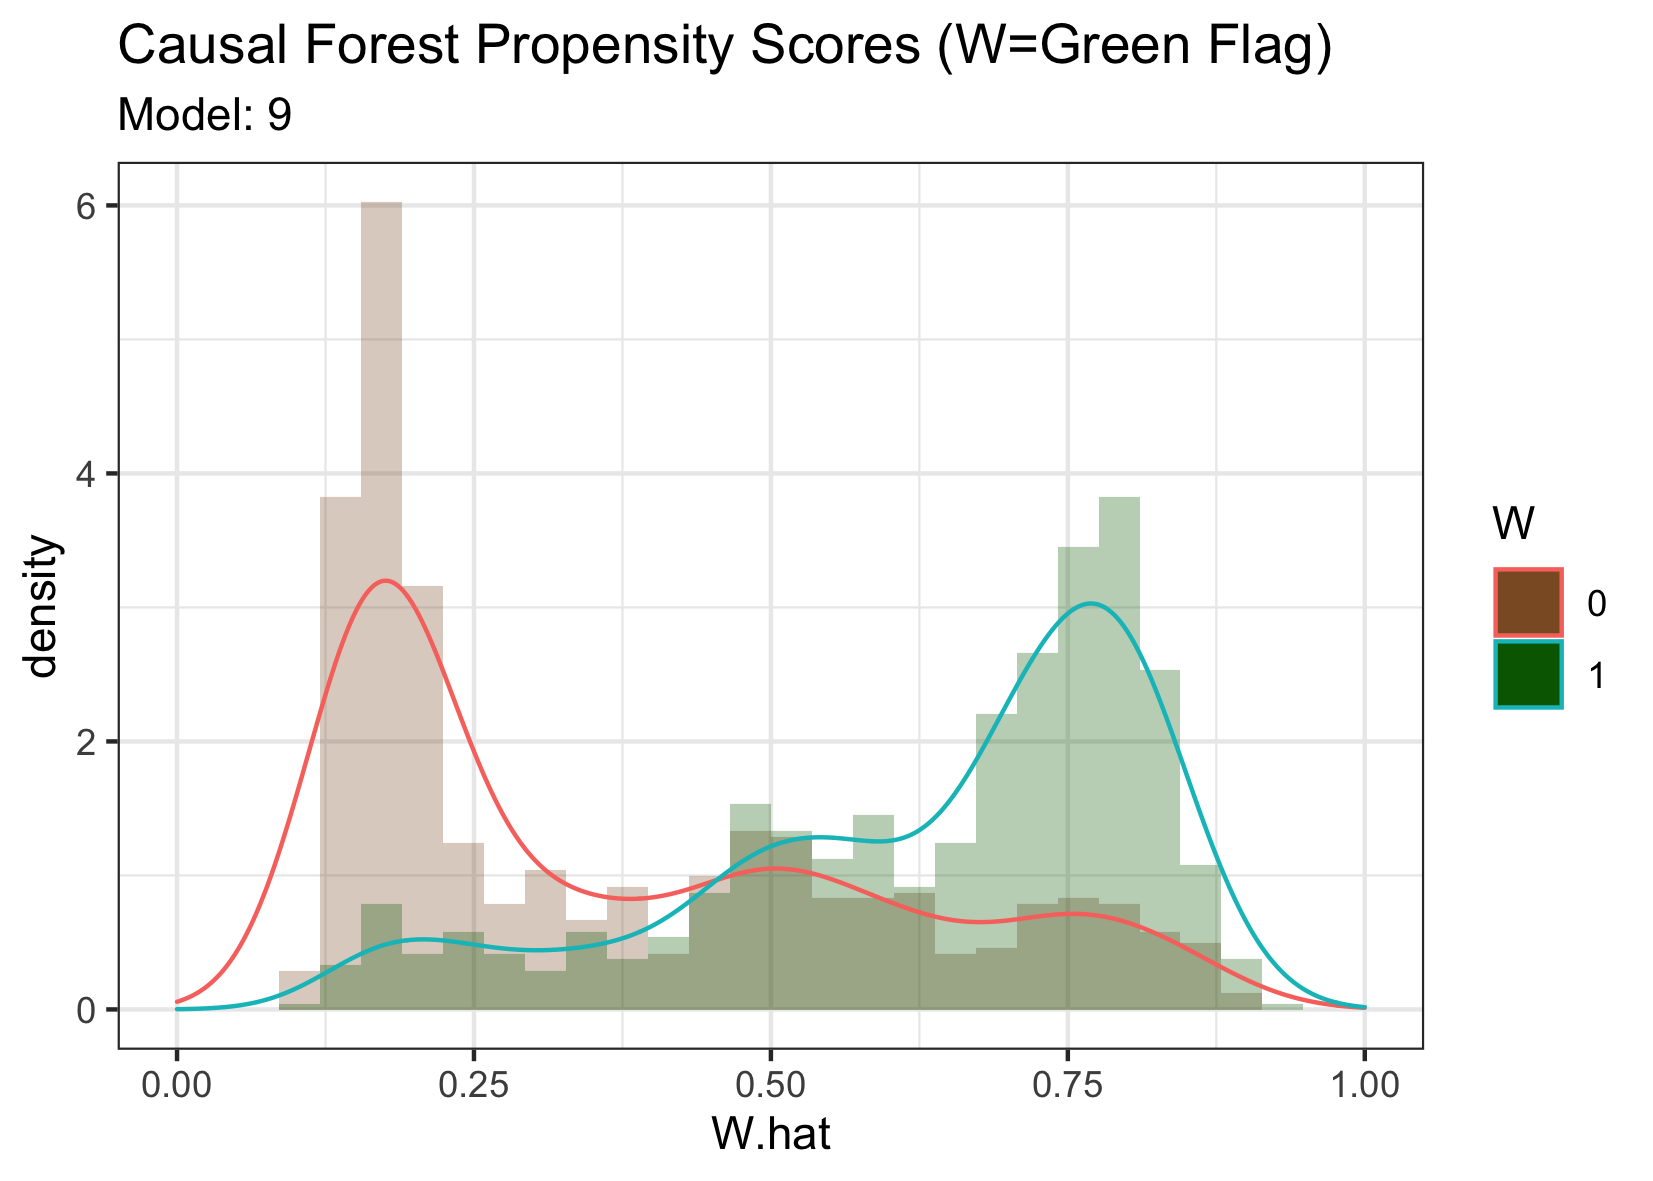
\includegraphics[scale=0.2]{chinchilab-template/chapters/appendices/ANALYSIS/prop_9.png}
    \caption{Propensity Score Distribution (Model 9)}
    \label{prop9}
\end{figure}

\begin{table}[H]{
    \begin{subtable}{.5\textwidth}
    \centering
    \footnotesize
        {\begin{tabular}{@{\extracolsep{5pt}}lc} 
        \\[-1.8ex]\hline 
        \hline \\[-1.8ex] 
         & \multicolumn{1}{c}{\textit{Dependent variable: Green Flag}} \\ 
        \cline{2-2} 
        \\[-1.8ex] &   \\ 
        \hline \\[-1.8ex] 
         e.bar & 1.004$^{***}$ \\ 
          & (0.023) \\ 
          & \\ 
         e.residual & 1.092$^{***}$ \\ 
          & (0.041) \\ 
          & \\ 
        \hline \\[-1.8ex] 
        \hline 
        \hline \\[-1.8ex] 
        \textit{Note:}  & \multicolumn{1}{r}{$^{*}$p$<$0.1; $^{**}$p$<$0.05; $^{***}$p$<$0.01} \\ 
        \end{tabular} }
    \subcaption{Outcome Model}
    \end{subtable}
    \begin{subtable}{0.3\linewidth}
    \centering
    \footnotesize
        {\begin{tabular}{@{\extracolsep{5pt}}lc} 
        \\[-1.8ex]\hline 
        \hline \\[-1.8ex] 
         & \multicolumn{1}{c}{\textit{Dependent variable: Green Flag}} \\ 
        \cline{2-2} 
        \\[-1.8ex] &   \\ 
        \hline \\[-1.8ex] 
         m.bar & 1.004$^{***}$ \\ 
          & (0.015) \\ 
          & \\ 
         m.residual & 1.313$^{***}$ \\ 
          & (0.031) \\ 
          & \\ 
        \hline \\[-1.8ex] 
        \hline 
        \hline \\[-1.8ex] 
        \textit{Note:}  & \multicolumn{1}{r}{$^{*}$p$<$0.1; $^{**}$p$<$0.05; $^{***}$p$<$0.01} \\ 
        \end{tabular} }
    \subcaption{Propensity Model}
    \end{subtable}
\caption{Calibration Regressions (Model 9)}
\label{calibration9}}
\end{table}

\newpage

%%%%%%%%%%%%%%%%%%%%%%%%%%%%%%%%%%%%%%%%%%%%%%%%%%%%%%%%%%%%
\subsubsection*{Heterogeneity Assessment}
%%%%%%%%%%%%%%%%%%%%%%%%%%%%%%%%%%%%%%%%%%%%%%%%%%%%%%%%%%%%

Again, we start by showing the distribution of CATEs in Figure \ref{cate9}. It can be noted that, compared to Figure \ref{cate4}, the distribution is more bell-formed with a central tendency around -0.3\% and -0.2\%.

\begin{figure}[H]
    \centering
    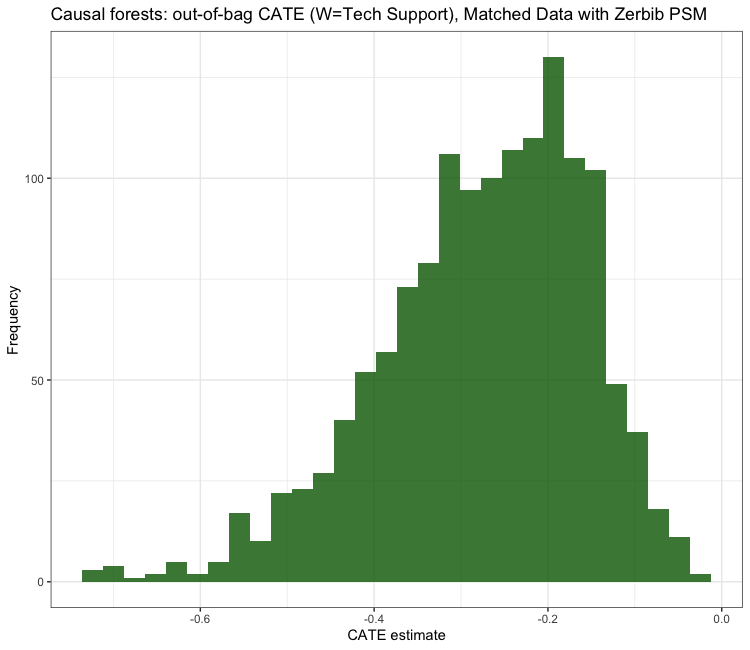
\includegraphics[scale=0.3]{chinchilab-template/chapters/appendices/ANALYSIS/CATE_cf22.png}
    \caption{Distribution of CATE (Model 9)}
    \label{cate9}
\end{figure}

The importance of the variables is shown in Table \ref{varimp9}. Similar to table \ref{varimp4}, the variables issue amount and time to maturity (days) are among the top 3 in importance.

\begin{table}[h!]
\centering
\caption{Variable Importance (Model 9)}
\label{varimp9}
\begin{tabular}{lr}
\\[-1.8ex]\hline 
\hline \\[-1.8ex]
\rowcolor[HTML]{FFFFFF} 
{\color[HTML]{333333} \textbf{Covariate}} & {\color[HTML]{333333} \textbf{Value}} \\ \hline
\rowcolor[HTML]{FFFFFF} 
{\color[HTML]{333333} Issue Amount} & \cellcolor[HTML]{00441B}{\color[HTML]{FFFFFF} 0.25640595} \\
\rowcolor[HTML]{FFFFFF} 
{\color[HTML]{333333} Time to Maturity (Days)} & \cellcolor[HTML]{268E47}{\color[HTML]{FFFFFF} 0.19958012} \\
\rowcolor[HTML]{FFFFFF} 
{\color[HTML]{333333} 2020} & \cellcolor[HTML]{D5EFCF}{\color[HTML]{333333} 0.08061582} \\
\rowcolor[HTML]{FFFFFF} 
{\color[HTML]{333333} 2018} & \cellcolor[HTML]{EDF8E9}{\color[HTML]{333333} 0.05449152} \\
\rowcolor[HTML]{FFFFFF} 
{\color[HTML]{333333} Financials} & \cellcolor[HTML]{F6FCF4}{\color[HTML]{333333} 0.04008215} \\
\rowcolor[HTML]{FFFFFF} 
{\color[HTML]{333333} 2022} & \cellcolor[HTML]{F7FCF5}{\color[HTML]{333333} 0.03899863} \\ \hline
\end{tabular}
\end{table}

Next, we show the mean ATE with error bound across quartiles in Figure \ref{quart9}. In contrast to Figure \ref{quart4}, the error bounds are larger and the overall range of the ATE is lower.

\begin{figure}[H]
    \centering
    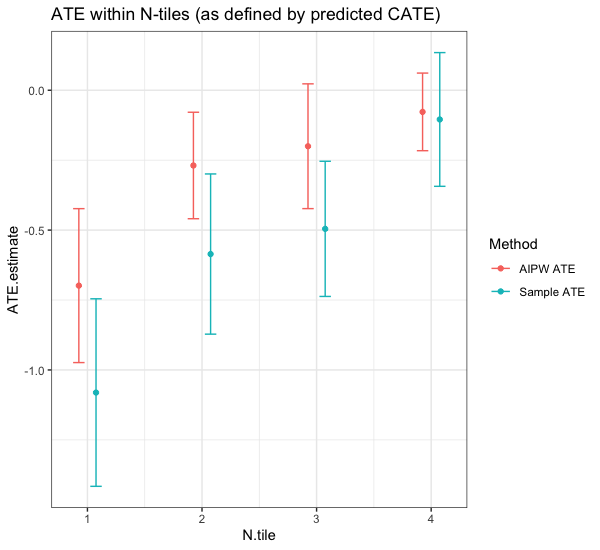
\includegraphics[scale=0.33]{chinchilab-template/chapters/appendices/ANALYSIS/ntile_cf22.png}
    \caption{Graph of ATE within Quartiles (Model 9)}
    \label{quart9}
\end{figure}

Also the heterogeneity across covariates shows a very similar pattern, compared to Table \ref{Het4}.

Next, the partial dependence plots are shown in Figure \ref{pdp9}. Here we can observe the first differences. First, the slope of the effect of the 2022 dummy is now almost horizontal, suggesting that the isolated effect of green bonds from 2022 is less pronounced compared to 2012. Second, both the issue amount and the time to maturity have a negative effect, in contrast to our previous observations.

\begin{figure}[H]
\centering
   \begin{subfigure}[b]{0.45\textwidth} \centering
    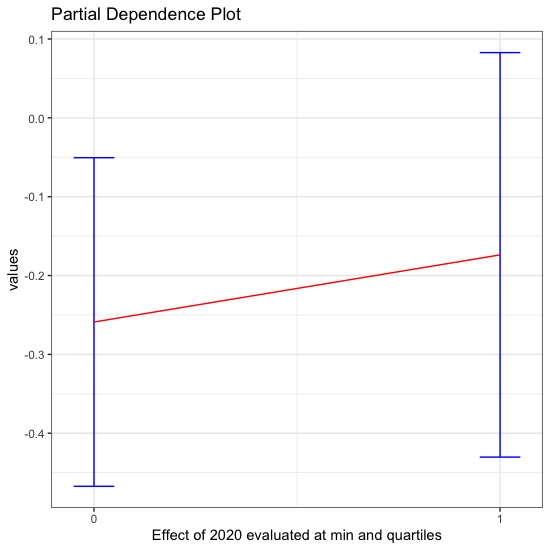
\includegraphics[width=0.65\textwidth]{chinchilab-template/chapters/appendices/ANALYSIS/PDP3_cf22.png}
    \caption{Effect of 2022}
   \label{fig:Ng1} 
\end{subfigure}
\begin{subfigure}[b]{0.5\textwidth} \centering
    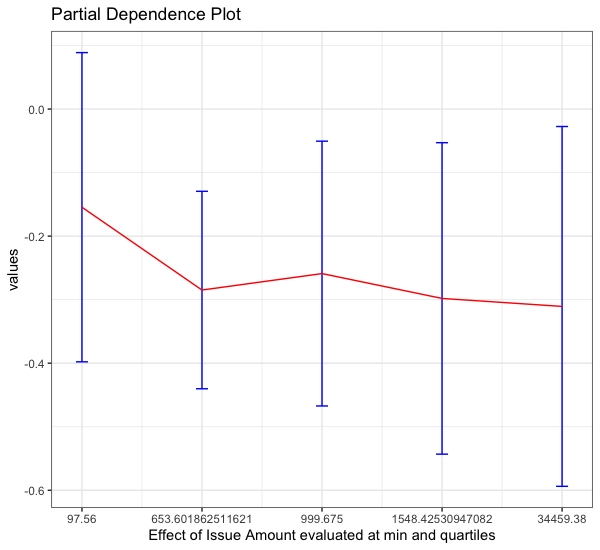
\includegraphics[width=0.65\textwidth]{chinchilab-template/chapters/appendices/ANALYSIS/PDP_cf22.png}
    \caption{Effect of Issue Amount}
   \label{fig:Ng2}
\end{subfigure}
\\
\begin{subfigure}[b]{0.5\textwidth} \centering
    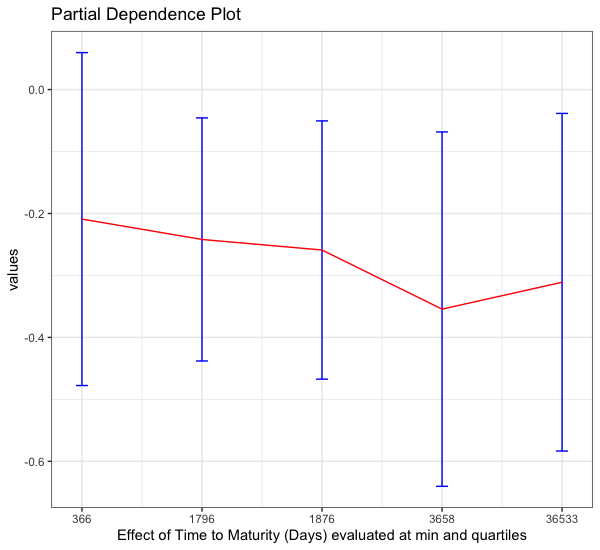
\includegraphics[width=0.65\textwidth]{chinchilab-template/chapters/appendices/ANALYSIS/PDP2_cf22.png}
    \caption{Effect of Time to Maturity (Days)}
   \label{fig:Ng2}
\end{subfigure}
\caption{Partial Dependence Plots (Model 9)}
\label{pdp9}
\end{figure}

\begin{table}[H]
\centering
\caption{Heterogeneity across Covariates (Model 9)}
\label{Het9}
\scriptsize
\begin{tabular}{lllll}
\\[-1.8ex]\hline 
\hline \\[-1.8ex] 
{\color[HTML]{333333} \textbf{Variable}} & {\color[HTML]{333333} \textbf{Mean ntile1}} & {\color[HTML]{333333} \textbf{Mean ntile2}} & {\color[HTML]{333333} \textbf{Mean ntile3}} & {\color[HTML]{333333} \textbf{Mean ntile4}} \\
\hline \\[-1.8ex] 
{\color[HTML]{333333} Time to Maturity (Days)} & \cellcolor[HTML]{A7DAB6}{\color[HTML]{333333} 2887.99} & \cellcolor[HTML]{63BE7B}{\color[HTML]{333333} 3733.21} & \cellcolor[HTML]{BBE2C7}{\color[HTML]{333333} 2633.11} & \cellcolor[HTML]{FCFCFF}{\color[HTML]{333333} 1810.53} \\
{\color[HTML]{333333} Issue   Amount} & \cellcolor[HTML]{6FC386}{\color[HTML]{333333} 1694.43} & \cellcolor[HTML]{81CB95}{\color[HTML]{333333} 1637.58} & \cellcolor[HTML]{FCFCFF}{\color[HTML]{333333} 1248.52} & \cellcolor[HTML]{63BE7B}{\color[HTML]{333333} 1731.59} \\
{\color[HTML]{333333} Guarantor} & \cellcolor[HTML]{DFF1E6}{\color[HTML]{333333} 0.19} & \cellcolor[HTML]{E1F1E7}{\color[HTML]{333333} 0.18} & \cellcolor[HTML]{EBF6F1}{\color[HTML]{333333} 0.11} & \cellcolor[HTML]{D7EDDF}{\color[HTML]{333333} 0.24} \\
{\color[HTML]{333333} 2013} & \cellcolor[HTML]{EBF6F1}{\color[HTML]{333333} 0.11} & \cellcolor[HTML]{F5F9F9}{\color[HTML]{333333} 0.05} & \cellcolor[HTML]{F5F9F9}{\color[HTML]{333333} 0.05} & \cellcolor[HTML]{F3F9F7}{\color[HTML]{333333} 0.06} \\
{\color[HTML]{333333} 2014} & \cellcolor[HTML]{EDF6F2}{\color[HTML]{333333} 0.1} & \cellcolor[HTML]{F3F9F7}{\color[HTML]{333333} 0.06} & \cellcolor[HTML]{F3F9F7}{\color[HTML]{333333} 0.06} & \cellcolor[HTML]{F5F9F9}{\color[HTML]{333333} 0.05} \\
{\color[HTML]{333333} 2015} & \cellcolor[HTML]{F3F9F7}{\color[HTML]{333333} 0.06} & \cellcolor[HTML]{EFF7F3}{\color[HTML]{333333} 0.09} & \cellcolor[HTML]{EFF7F3}{\color[HTML]{333333} 0.09} & \cellcolor[HTML]{F3F9F7}{\color[HTML]{333333} 0.06} \\
{\color[HTML]{333333} 2016} & \cellcolor[HTML]{F0F7F5}{\color[HTML]{333333} 0.08} & \cellcolor[HTML]{F0F7F5}{\color[HTML]{333333} 0.08} & \cellcolor[HTML]{F2F8F6}{\color[HTML]{333333} 0.07} & \cellcolor[HTML]{F0F7F5}{\color[HTML]{333333} 0.08} \\
{\color[HTML]{333333} 2017} & \cellcolor[HTML]{F9FBFD}{\color[HTML]{333333} 0.02} & \cellcolor[HTML]{EBF6F1}{\color[HTML]{333333} 0.11} & \cellcolor[HTML]{EDF6F2}{\color[HTML]{333333} 0.1} & \cellcolor[HTML]{F2F8F6}{\color[HTML]{333333} 0.07} \\
{\color[HTML]{333333} 2018} & \cellcolor[HTML]{FCFCFF}{\color[HTML]{333333} 0} & \cellcolor[HTML]{F0F7F5}{\color[HTML]{333333} 0.08} & \cellcolor[HTML]{E8F4EE}{\color[HTML]{333333} 0.13} & \cellcolor[HTML]{F2F8F6}{\color[HTML]{333333} 0.07} \\
{\color[HTML]{333333} 2019} & \cellcolor[HTML]{F8FBFB}{\color[HTML]{333333} 0.03} & \cellcolor[HTML]{E8F4EE}{\color[HTML]{333333} 0.13} & \cellcolor[HTML]{EBF6F1}{\color[HTML]{333333} 0.11} & \cellcolor[HTML]{F6FAFA}{\color[HTML]{333333} 0.04} \\
{\color[HTML]{333333} 2020} & \cellcolor[HTML]{FBFCFE}{\color[HTML]{333333} 0.01} & \cellcolor[HTML]{EFF7F3}{\color[HTML]{333333} 0.09} & \cellcolor[HTML]{EFF7F3}{\color[HTML]{333333} 0.09} & \cellcolor[HTML]{F0F7F5}{\color[HTML]{333333} 0.08} \\
{\color[HTML]{333333} 2021} & \cellcolor[HTML]{F5F9F9}{\color[HTML]{333333} 0.05} & \cellcolor[HTML]{EFF7F3}{\color[HTML]{333333} 0.09} & \cellcolor[HTML]{EFF7F3}{\color[HTML]{333333} 0.09} & \cellcolor[HTML]{F6FAFA}{\color[HTML]{333333} 0.04} \\
{\color[HTML]{333333} 2022} & \cellcolor[HTML]{FCFCFF}{\color[HTML]{333333} 0} & \cellcolor[HTML]{FCFCFF}{\color[HTML]{333333} 0} & \cellcolor[HTML]{FCFCFF}{\color[HTML]{333333} 0} & \cellcolor[HTML]{D4ECDD}{\color[HTML]{333333} 0.26} \\
{\color[HTML]{333333} Annual Coupon} & \cellcolor[HTML]{63BE7B}{\color[HTML]{333333} 0.99} & \cellcolor[HTML]{79C78E}{\color[HTML]{333333} 0.85} & \cellcolor[HTML]{ABDBB9}{\color[HTML]{333333} 0.53} & \cellcolor[HTML]{E1F1E7}{\color[HTML]{333333} 0.18} \\
{\color[HTML]{333333} Semi Annual Coupon} & \cellcolor[HTML]{FBFCFE}{\color[HTML]{333333} 0.01} & \cellcolor[HTML]{E5F3EB}{\color[HTML]{333333} 0.15} & \cellcolor[HTML]{B4DFC1}{\color[HTML]{333333} 0.47} & \cellcolor[HTML]{7EC992}{\color[HTML]{333333} 0.82} \\
{\color[HTML]{333333} Quarterly} & \cellcolor[HTML]{FCFCFF}{\color[HTML]{333333} 0} & \cellcolor[HTML]{FCFCFF}{\color[HTML]{333333} 0} & \cellcolor[HTML]{FCFCFF}{\color[HTML]{333333} 0} & \cellcolor[HTML]{FCFCFF}{\color[HTML]{333333} 0} \\
{\color[HTML]{333333} Senior Secured Mortgage} & \cellcolor[HTML]{FCFCFF}{\color[HTML]{333333} 0} & \cellcolor[HTML]{E1F1E7}{\color[HTML]{333333} 0.18} & \cellcolor[HTML]{EBF6F1}{\color[HTML]{333333} 0.11} & \cellcolor[HTML]{F5F9F9}{\color[HTML]{333333} 0.05} \\
{\color[HTML]{333333} Senior Secured} & \cellcolor[HTML]{F9FBFD}{\color[HTML]{333333} 0.02} & \cellcolor[HTML]{EDF6F2}{\color[HTML]{333333} 0.1} & \cellcolor[HTML]{F6FAFA}{\color[HTML]{333333} 0.04} & \cellcolor[HTML]{F3F9F7}{\color[HTML]{333333} 0.06} \\
{\color[HTML]{333333} Senior Unsecured} & \cellcolor[HTML]{76C68B}{\color[HTML]{333333} 0.87} & \cellcolor[HTML]{ABDBB9}{\color[HTML]{333333} 0.53} & \cellcolor[HTML]{B1DEBE}{\color[HTML]{333333} 0.49} & \cellcolor[HTML]{89CE9B}{\color[HTML]{333333} 0.75} \\
{\color[HTML]{333333} Senior Non Preferred} & \cellcolor[HTML]{FCFCFF}{\color[HTML]{333333} 0} & \cellcolor[HTML]{F9FBFD}{\color[HTML]{333333} 0.02} & \cellcolor[HTML]{EFF7F3}{\color[HTML]{333333} 0.09} & \cellcolor[HTML]{F9FBFD}{\color[HTML]{333333} 0.02} \\
{\color[HTML]{333333} Senior Preferred} & \cellcolor[HTML]{FCFCFF}{\color[HTML]{333333} 0} & \cellcolor[HTML]{F8FBFB}{\color[HTML]{333333} 0.03} & \cellcolor[HTML]{E7F4ED}{\color[HTML]{333333} 0.14} & \cellcolor[HTML]{F6FAFA}{\color[HTML]{333333} 0.04} \\
{\color[HTML]{333333} Senior Subordinated Unsecured} & \cellcolor[HTML]{FBFCFE}{\color[HTML]{333333} 0.01} & \cellcolor[HTML]{FCFCFF}{\color[HTML]{333333} 0} & \cellcolor[HTML]{FCFCFF}{\color[HTML]{333333} 0} & \cellcolor[HTML]{FCFCFF}{\color[HTML]{333333} 0} \\
{\color[HTML]{333333} Subordinated Unsecured} & \cellcolor[HTML]{FBFCFE}{\color[HTML]{333333} 0.01} & \cellcolor[HTML]{F9FBFD}{\color[HTML]{333333} 0.02} & \cellcolor[HTML]{F6FAFA}{\color[HTML]{333333} 0.04} & \cellcolor[HTML]{FCFCFF}{\color[HTML]{333333} 0} \\
{\color[HTML]{333333} Basic Materials} & \cellcolor[HTML]{FBFCFE}{\color[HTML]{333333} 0.01} & \cellcolor[HTML]{FCFCFF}{\color[HTML]{333333} 0} & \cellcolor[HTML]{FCFCFF}{\color[HTML]{333333} 0} & \cellcolor[HTML]{FCFCFF}{\color[HTML]{333333} 0} \\
{\color[HTML]{333333} Consumer Cyclicals} & \cellcolor[HTML]{F9FBFD}{\color[HTML]{333333} 0.02} & \cellcolor[HTML]{FCFCFF}{\color[HTML]{333333} 0} & \cellcolor[HTML]{FCFCFF}{\color[HTML]{333333} 0} & \cellcolor[HTML]{FCFCFF}{\color[HTML]{333333} 0} \\
{\color[HTML]{333333} Consumer Non Cyclicals} & \cellcolor[HTML]{FCFCFF}{\color[HTML]{333333} 0} & \cellcolor[HTML]{FCFCFF}{\color[HTML]{333333} 0} & \cellcolor[HTML]{FCFCFF}{\color[HTML]{333333} 0} & \cellcolor[HTML]{FCFCFF}{\color[HTML]{333333} 0} \\
{\color[HTML]{333333} Energy} & \cellcolor[HTML]{F9FBFD}{\color[HTML]{333333} 0.02} & \cellcolor[HTML]{FCFCFF}{\color[HTML]{333333} 0} & \cellcolor[HTML]{FCFCFF}{\color[HTML]{333333} 0} & \cellcolor[HTML]{FCFCFF}{\color[HTML]{333333} 0} \\
{\color[HTML]{333333} Financials} & \cellcolor[HTML]{ACDCBA}{\color[HTML]{333333} 0.52} & \cellcolor[HTML]{9ED6AE}{\color[HTML]{333333} 0.61} & \cellcolor[HTML]{8DCF9F}{\color[HTML]{333333} 0.72} & \cellcolor[HTML]{81CA95}{\color[HTML]{333333} 0.8} \\
{\color[HTML]{333333} Healthcare} & \cellcolor[HTML]{FCFCFF}{\color[HTML]{333333} 0} & \cellcolor[HTML]{FCFCFF}{\color[HTML]{333333} 0} & \cellcolor[HTML]{FCFCFF}{\color[HTML]{333333} 0} & \cellcolor[HTML]{FCFCFF}{\color[HTML]{333333} 0} \\
{\color[HTML]{333333} Industrials} & \cellcolor[HTML]{F9FBFD}{\color[HTML]{333333} 0.02} & \cellcolor[HTML]{F9FBFD}{\color[HTML]{333333} 0.02} & \cellcolor[HTML]{F9FBFD}{\color[HTML]{333333} 0.02} & \cellcolor[HTML]{FCFCFF}{\color[HTML]{333333} 0} \\
{\color[HTML]{333333} Institutions, Associations \& Organizations} & \cellcolor[HTML]{F8FBFB}{\color[HTML]{333333} 0.03} & \cellcolor[HTML]{F6FAFA}{\color[HTML]{333333} 0.04} & \cellcolor[HTML]{F2F8F6}{\color[HTML]{333333} 0.07} & \cellcolor[HTML]{F8FBFB}{\color[HTML]{333333} 0.03} \\
{\color[HTML]{333333} Real Estate} & \cellcolor[HTML]{FCFCFF}{\color[HTML]{333333} 0} & \cellcolor[HTML]{FCFCFF}{\color[HTML]{333333} 0} & \cellcolor[HTML]{FCFCFF}{\color[HTML]{333333} 0} & \cellcolor[HTML]{FCFCFF}{\color[HTML]{333333} 0} \\
{\color[HTML]{333333} Technology} & \cellcolor[HTML]{F8FBFB}{\color[HTML]{333333} 0.03} & \cellcolor[HTML]{FCFCFF}{\color[HTML]{333333} 0} & \cellcolor[HTML]{FCFCFF}{\color[HTML]{333333} 0} & \cellcolor[HTML]{FCFCFF}{\color[HTML]{333333} 0} \\
{\color[HTML]{333333} Utilities} & \cellcolor[HTML]{F6FAFA}{\color[HTML]{333333} 0.04} & \cellcolor[HTML]{FBFCFE}{\color[HTML]{333333} 0.01} & \cellcolor[HTML]{FBFCFE}{\color[HTML]{333333} 0.01} & \cellcolor[HTML]{FBFCFE}{\color[HTML]{333333} 0.01} \\
{\color[HTML]{333333} AAA} & \cellcolor[HTML]{CDE9D6}{\color[HTML]{333333} 0.31} & \cellcolor[HTML]{AEDDBB}{\color[HTML]{333333} 0.51} & \cellcolor[HTML]{C3E5CE}{\color[HTML]{333333} 0.37} & \cellcolor[HTML]{A7DAB6}{\color[HTML]{333333} 0.55} \\
{\color[HTML]{333333} AA} & \cellcolor[HTML]{D1EBDA}{\color[HTML]{333333} 0.28} & \cellcolor[HTML]{D3ECDB}{\color[HTML]{333333} 0.27} & \cellcolor[HTML]{DFF1E6}{\color[HTML]{333333} 0.19} & \cellcolor[HTML]{CDE9D6}{\color[HTML]{333333} 0.31} \\
{\color[HTML]{333333} A} & \cellcolor[HTML]{DEF0E5}{\color[HTML]{333333} 0.2} & \cellcolor[HTML]{EDF6F2}{\color[HTML]{333333} 0.1} & \cellcolor[HTML]{DCEFE3}{\color[HTML]{333333} 0.21} & \cellcolor[HTML]{EFF7F3}{\color[HTML]{333333} 0.09} \\
{\color[HTML]{333333} BBB} & \cellcolor[HTML]{DFF1E6}{\color[HTML]{333333} 0.19} & \cellcolor[HTML]{EBF6F1}{\color[HTML]{333333} 0.11} & \cellcolor[HTML]{DEF0E5}{\color[HTML]{333333} 0.2} & \cellcolor[HTML]{F5F9F9}{\color[HTML]{333333} 0.05} \\
{\color[HTML]{333333} BB} & \cellcolor[HTML]{F9FBFD}{\color[HTML]{333333} 0.02} & \cellcolor[HTML]{FCFCFF}{\color[HTML]{333333} 0} & \cellcolor[HTML]{F9FBFD}{\color[HTML]{333333} 0.02} & \cellcolor[HTML]{FCFCFF}{\color[HTML]{333333} 0} \\
{\color[HTML]{333333} AUD} & \cellcolor[HTML]{FBFCFE}{\color[HTML]{333333} 0.01} & \cellcolor[HTML]{F6FAFA}{\color[HTML]{333333} 0.04} & \cellcolor[HTML]{FCFCFF}{\color[HTML]{333333} 0} & \cellcolor[HTML]{FCFCFF}{\color[HTML]{333333} 0} \\
{\color[HTML]{333333} CAD} & \cellcolor[HTML]{FCFCFF}{\color[HTML]{333333} 0} & \cellcolor[HTML]{F9FBFD}{\color[HTML]{333333} 0.02} & \cellcolor[HTML]{FBFCFE}{\color[HTML]{333333} 0.01} & \cellcolor[HTML]{FCFCFF}{\color[HTML]{333333} 0} \\
{\color[HTML]{333333} CLP} & \cellcolor[HTML]{FCFCFF}{\color[HTML]{333333} 0} & \cellcolor[HTML]{FCFCFF}{\color[HTML]{333333} 0} & \cellcolor[HTML]{FCFCFF}{\color[HTML]{333333} 0} & \cellcolor[HTML]{FCFCFF}{\color[HTML]{333333} 0} \\
{\color[HTML]{333333} CNY} & \cellcolor[HTML]{FCFCFF}{\color[HTML]{333333} 0} & \cellcolor[HTML]{FCFCFF}{\color[HTML]{333333} 0} & \cellcolor[HTML]{FCFCFF}{\color[HTML]{333333} 0} & \cellcolor[HTML]{FCFCFF}{\color[HTML]{333333} 0} \\
{\color[HTML]{333333} EUR} & \cellcolor[HTML]{6DC283}{\color[HTML]{333333} 0.93} & \cellcolor[HTML]{8ACE9D}{\color[HTML]{333333} 0.74} & \cellcolor[HTML]{CBE8D5}{\color[HTML]{333333} 0.32} & \cellcolor[HTML]{E4F2EA}{\color[HTML]{333333} 0.16} \\
{\color[HTML]{333333} GBP} & \cellcolor[HTML]{F3F9F7}{\color[HTML]{333333} 0.06} & \cellcolor[HTML]{E8F4EE}{\color[HTML]{333333} 0.13} & \cellcolor[HTML]{F8FBFB}{\color[HTML]{333333} 0.03} & \cellcolor[HTML]{FBFCFE}{\color[HTML]{333333} 0.01} \\
{\color[HTML]{333333} HKD} & \cellcolor[HTML]{FCFCFF}{\color[HTML]{333333} 0} & \cellcolor[HTML]{FCFCFF}{\color[HTML]{333333} 0} & \cellcolor[HTML]{FCFCFF}{\color[HTML]{333333} 0} & \cellcolor[HTML]{FCFCFF}{\color[HTML]{333333} 0} \\
{\color[HTML]{333333} JPY} & \cellcolor[HTML]{FCFCFF}{\color[HTML]{333333} 0} & \cellcolor[HTML]{F8FBFB}{\color[HTML]{333333} 0.03} & \cellcolor[HTML]{F5F9F9}{\color[HTML]{333333} 0.05} & \cellcolor[HTML]{FCFCFF}{\color[HTML]{333333} 0} \\
{\color[HTML]{333333} NZD} & \cellcolor[HTML]{FCFCFF}{\color[HTML]{333333} 0} & \cellcolor[HTML]{FCFCFF}{\color[HTML]{333333} 0} & \cellcolor[HTML]{FCFCFF}{\color[HTML]{333333} 0} & \cellcolor[HTML]{FCFCFF}{\color[HTML]{333333} 0} \\
{\color[HTML]{333333} NOK} & \cellcolor[HTML]{FCFCFF}{\color[HTML]{333333} 0} & \cellcolor[HTML]{FCFCFF}{\color[HTML]{333333} 0} & \cellcolor[HTML]{FCFCFF}{\color[HTML]{333333} 0} & \cellcolor[HTML]{FCFCFF}{\color[HTML]{333333} 0} \\
{\color[HTML]{333333} SEK} & \cellcolor[HTML]{FCFCFF}{\color[HTML]{333333} 0} & \cellcolor[HTML]{FBFCFE}{\color[HTML]{333333} 0.01} & \cellcolor[HTML]{FCFCFF}{\color[HTML]{333333} 0} & \cellcolor[HTML]{FCFCFF}{\color[HTML]{333333} 0} \\
{\color[HTML]{333333} UYU} & \cellcolor[HTML]{FCFCFF}{\color[HTML]{333333} 0} & \cellcolor[HTML]{FCFCFF}{\color[HTML]{333333} 0} & \cellcolor[HTML]{FCFCFF}{\color[HTML]{333333} 0} & \cellcolor[HTML]{FCFCFF}{\color[HTML]{333333} 0}
\end{tabular}
\end{table}

Finally, both results of the USDEUR and CBI subsets show a very similar pattern to the one we described above.
\newpage

\section{Monte-Carlo Simulation}

In a Monte Carlo simulation, the data used for the analysis is simulated. The baseline model of interest can be described as follows:

\begin{equation*}
y = dy^{1} + (1-d)y^{0}
\end{equation*}

\subsection*{DGP 1}
In the first DGP the model of interest can be described as follows:

    \begin{align*}
        &y^0 \sim \text{CIR}^N \\
        &y^1 = 0.1 + g(\textbf{X}^{N\times K}) + \text{CIR}^N, \quad \text{where} \quad \textbf{X}^{N\times K} \sim \mathcal{N}(0,1) \\
        &g(\textbf{X}^{N\times K}) = \textbf{X'}^{N\times K} \beta \quad \text{where} \quad \beta = (1/K,...,K/K) \\
        &d \sim \mathcal{B}(p=0.2) \\
    \end{align*}

where $\text{CIR}^N$ is a vector of interest rates generated by the Cox-Ingersoll-Ross (CIR) process. This process is used when calculating the evolution of interest rates. Mathematically, it has the following form \citep[p. 391]{cox2005theory}:

\begin{equation}
d r_t=a\left(b-r_t\right) d t+\sigma \sqrt{r_t} d W_t
\end{equation}

Here, $a$, $b$, and $\sigma$ are positive constants, $r_t$ is the interest rate, $t$ is the time, and $W_t$ denotes the standard Wiener process. Moreover, as can be seen from the first term, the process is mean-reverting, where $b$ is the long-run average interest rate, and $a$ is the speed of adjustment. Moreover, $\sigma$ is the volatility.

For this simple DGP all identifying assumptions are fulfilled such that we can estimate an unbiased ATE as $E[y_i^{1}-y_i^{0}]=0.1$.

\subsection*{DGP 2}

The second DGP is very similar to the first, with the exception that we allow the i.i.d assumption of the outcome to be violated. In order to do that we add an issuer dependency vector to the $\text{CIR}^N$ vector. The rationale being that bond returns are not generated in an i.i.d. process, but in a process that depends on the issuer. Therefore, we generate a random subset of issuers where each unique issuer receives a randomly assigned issuer effect. In this way, we are also able to adjust the intensity of the dependency.

\subsection*{Results}

The following histograms show the empirical distribution of our estimated ATE for both DGPs. Please note that we set $K$, the number of observable confounders to $10$ and the number of
observations to $N = 1'000$. The other parameters can be found in the code in the appendix.

First, Figure \ref{LIE} shows the results for a relatively small issuer effect. We can note that the causal forest captures the ATE distribution very similarly for both DGPs. Thus, if the dependence effect is small, there is no cost to estimation performance.

\begin{figure}[H]
    \centering
    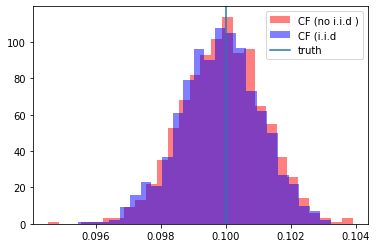
\includegraphics[scale=0.6]{chinchilab-template/chapters/chapter04/dgp1.png}
    \caption{Low Issuer Effect}
    \label{LIE}
\end{figure}

However, Figure \ref{HIE} displays the results for a high issuer effect. In particular, this effect is five times higher as before. We can observe a difference in the distributions, namely that the ATE estimate of our DGP violating the i.i.d assumption has a higher variance compared to Figure \ref{LIE}. Thus, we conclude that violating the i.i.d. assumption only has a negative effect on the estimation accuracy of the causal forest. However, this negative effect is only marginal. Moreover, since we could argue that this dependence effect is relatively small in reality, the effect is approximately zero, as suggested by Figure \ref{LIE}.

\begin{figure}[H]
    \centering
    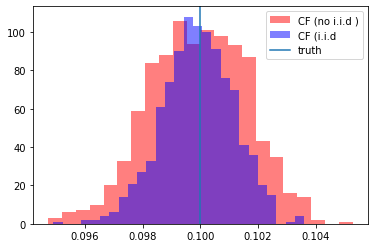
\includegraphics[scale=0.6]{chinchilab-template/chapters/chapter04/dgp2.png}
    \caption{High Issuer Effect}
    \label{HIE}
\end{figure}